\section{Kondensierte Materie 2}
\subsection{Dielektrische und optische Eigenschaften}
\noindent\textbf{1. Welcher Zusammenhang besteht zwischen der dielektrischen Funktion und den optischen Eigenschaften eines Festkörpers?}\\
\begin{addmargin}[25pt]{0pt}
Die dielektrische Funktion $\varepsilon$ kann aufgeteilt werden in einen Realteil $\varepsilon'$ und einen Imaginärteil $\varepsilon''$. Der direkte Zusammenhang mit den optischen Eigenschaften ist, dass das Quadrat des komplexen Brechungsindexes $n = n' + i\kappa$ gleich der dielektrischen Funktion entspricht:
\begin{equation}\label{eq:epsilon_n}
    \varepsilon' + i\varepsilon'' = (n' + i\kappa)^2
\end{equation}
oder ausmultipliziert:
\begin{align}
    \varepsilon' &= n'^2 -\kappa^2\\
    \varepsilon'' &= 2n'\kappa
\end{align}
Aus dieser Eigenschaft folgt direkt die Verbindung von $\varepsilon$ mit dem Reflexionsgrad $R$:
\begin{equation}\label{eq:epsilon_R}
    R = \left| \frac{\sqrt{\varepsilon} - 1}{\sqrt{\varepsilon} + 1}\right|^2
\end{equation}
\end{addmargin}

\noindent\textbf{2. Welches elektrische Feld wirkt lokal an der Position eines Atoms in einem polarisierbaren Festkörper, der sich in einem homogenen äußeren elektrischen Feld befindet?}\\
\begin{addmargin}[25pt]{0pt}
An dieser Position wirkt sowohl das äußere elektrische Feld $\mathbf{E}_a$ als auch ein elektrisches Feld aufgrund der im Festkörper relativ nahen Nachbaratome. Die Summe dieser Beiträge heißt lokales Feld $\mathbf{E}_{lok}$. In genauerer Betrachtung weißt das lokale Feld 4 Komponenten auf. Eine dieser Komponenten ist das äußere Feld $\mathbf{E}_a$ selbst. Eine zweite Komponente ist das Depolarisationsfeld $\mathbf{E}_D$, das entsteht ,da im gesamten Festkörper die Atome polarisiert werden und so an der Oberfläche des Körpers eine induzierte Oberflächenladung erzeugt wird. Das Feld dieser Ladung wirkt dem äußeren Feld entgegen. Ein dritter Beitrag ist das Lorentzfeld $\mathbf{E}_L$. Dieses entsteht da jedes Atom, also insbesondere auch die nah am Betrachtungsort des lokalen Feldes, polarisiert sind. Durch diese Dipole entsteht das Lorentzfeld $\mathbf{E}_L = \frac{1}{3\varepsilon_0}\mathbf{P}$. $\mathbf{P}$ ist die Polarisierung des Körpers. Der letzte Beitrag zum lokalen Feld ist die direkte Wirkung von benachbarten Atomen. Diese werden ohne Polarisierung betrachtet. Dieser Teil ist, bei Summation über alle Nachbarn, aus Symmetriegründen ungefähr null. \\
\end{addmargin}

\noindent\textbf{3. Wie können wir Festkörper hinsichtlich ihrer Reaktion auf äußere elektrische Felder klassifizieren?}\\
\begin{addmargin}[25pt]{0pt}
Man kann Festkörper einteilen in dielektrische, paraelektrische und ferro- bzw. antiferroelektrische Festkörper. Dielektrische Festkörper bilden unter dem Einfluss externer Felder im atomaren Bereich Dipole aus. Diese Dipole entstehen entweder durch Verschiebung der Elektronenwolke um den Atomkern oder durch Verschiebung der Ionen relativ zueinander. In paraelektrischen Materialien treten auch ohne äußeres Feld bereits Dipole auf, diese sind allerdings ungeordnet, wodurch kein makroskopisches elektrisches Feld messbar ist. Sobald ein äußeres elektrisches Feld angelegt wird orientieren sich diese Dipole alle in eine Richtung und man misst ein elektrisches Feld aufgrund dieser \textit{Orientierungspolarisation}. In ferroelektrischen Materialien tritt auch ohne äußeres Feld eine Polarisation auf. \\
\end{addmargin}

\noindent\textbf{4. Was beschreibt das Lorentz'sche Oszillatormodell?}\\
\begin{addmargin}[25pt]{0pt}
    Das Lorentz'sche Oszillatormodell wird angenommen, dass die an einem Atomkern gebundenen Elektronen sich so verhalten, als wären sie mit einer Feder am Atomkern befestigt. Durch äußere Bestrahlung mit Licht, dessen $\mathbf{E}$-Feld Komponente harmonisch oszilliert, wird das Elektron zum Schwingen angeregt und aus der Auslenkung kann die Polarisierbarkeit bestimmen werden.  \\
\end{addmargin}

\noindent\textbf{5. Was ist ein Polariton?}\\
\begin{addmargin}[25pt]{0pt}
Das Polariton ist ein Quasiteilchen, welches entsteht wenn ein elektromagnetisches Feld an ein transversal-optisches-Phonon koppelt. Bei starker Kopplung zwischen Phonon und Photon kann man den Prozess nicht mehr mit der Störungstheorie beschreiben. In diesem Fall  wird das Polariton benötigt um die Anregung zu beschreiben. In ionischen Kristallen ruft das Photon eine lokale Polarisation hervor, welche gleichbedeutend mit einer Gitterverzerrung ist. Diese Gitterverzerrung wird durch das Polariton beschrieben. Polaritonen entstehen in ionischen Kristallen.\\
\end{addmargin}

\noindent\textbf{6. Wie verhält sich die Dispersionsrelation eines Polaritons für $\omega < \omega_t$ und $\omega > \omega_l$?}\\
\begin{addmargin}[25pt]{0pt}
Für ganz kleine Frequenzen kann der Kristall aufgrund der geringen Energie des Lichts nicht zu Schwingungen angeregt werden, die Dispersionsrelation verhält sich also wie die von Photonen. Mit steigender Frequenz (bis zu $\omega_t$) werden immer mehr Gitterschwingungen angeregt bis sich die Polaritonen bei $\omega = \omega_t$ wie transversal-optische Phononen verhalten. Für Frequenzen $\omega >\omega_l$ werden erst nur Schwingungen angeregt also verhalten sich die Polaritonen wie Phononen. Bei noch höheren Frequenzen verhalten sie sich wieder wie Photonen weil das Licht so hochfrequent ist, dass keine Schwingungen angeregt werden können.   \\
\end{addmargin}

\noindent\textbf{7. Was passiert im Bereich $\omega_t < \omega < \omega_l$?}\\
\begin{addmargin}[25pt]{0pt}
Licht mit dieser Frequenz kann sich im Körper nicht ausbreiten, das Licht wird totalreflektiert. Dadurch gibt es im Festkörper weder Photonen noch Gitterschwingungen, wodurch auch keine Polaritonen entstehen.\\
\end{addmargin}

\noindent\textbf{8. Was sind Plasmonen?}\\
\begin{addmargin}[25pt]{0pt}
Das Plasmon ist das Quasiteilchen der Plasmaschwingung. Es beschreibt die Schwingung in einem Plasma, wie zum Beispiel die Oszillationen der Dichte in einem freien Elektronengas. Plasmonen können, ähnlich wie Phononen, an Photonen koppeln, dabei entsteht dann ein Plasmon-Polariton. \\
\end{addmargin}



\subsection{Halbleiter}
\subsubsection{Kurzfragen basierend auf den Übungsblättern von Professor Back}
\noindent\textbf{1. Wie kann man aus der Formel für die Stromdichte an einem pn-Übergang die Sperrrichtung und die Durchlassrichtung erkennen?}\\
\begin{addmargin}[25pt]{0pt}
 Für die Stromdichte an einem pn-Übergang gilt:
 \begin{equation}\label{eq:Strom_pn_transition}
      j(U) \propto \exp(\frac{eU}{k_BT}) -1
 \end{equation}
 Man kann anhand von Gleichung \ref{eq:Strom_pn_transition} erkennen, dass bei $U<0$ die Exponentialfunktion eine Wert zwischen null und eins annimmt, die Stromdichte ist somit für jeden Wert von $U$ relativ klein. Im Fall von $U>0$ also der Durchlassrichtung wird der Strom sehr schnell sehr stark ansteigen.   
 \end{addmargin}


\noindent\textbf{2. Wie sieht die Strom-Spannungskennlinie für einen pn-Übergang aus?}\\
\begin{addmargin}[25pt]{0pt}
\begin{figure}[h]
    \centering
    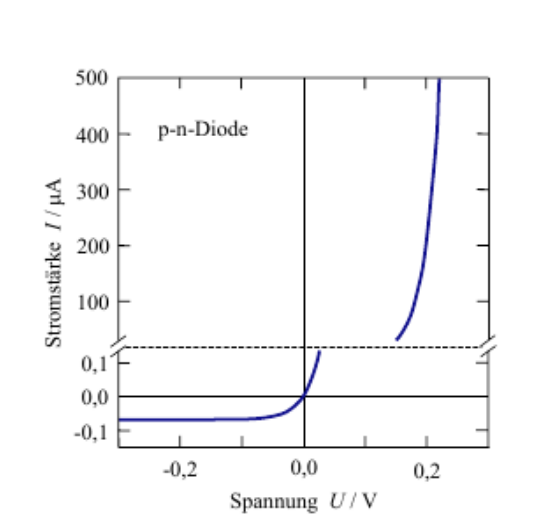
\includegraphics[width = 0.8\textwidth]{images/KM2/pn_transition_Strom_Spannung.png}
    \caption{Verlauf des Stroms in Abhängigkeit der Spnnung am pn-Übergang}
    \label{fig:pn_transition_Strom_Spannung}
\end{figure} 
Die Strom-Spannungskennlinie ist in Abbildung \ref{fig:pn_transition_Strom_Spannung} dargestellt. Man erkennt, dass in der Durchlassrichtung, also $U>0$ der Stromfluss um mehrere Größenordnungen höher ist als in der Sperrrichtung.\\
 \end{addmargin}

\noindent\textbf{3. Wie sieht das Banddiagramm für eine Schottky-Barriere aus für den Fall, dass Metall und Halbleiter voneinander getrennt sind und für den Fall dass sie in Kontakt stehen?}\\
\begin{addmargin}[25pt]{0pt}
    \begin{figure}[h]
        \centering
        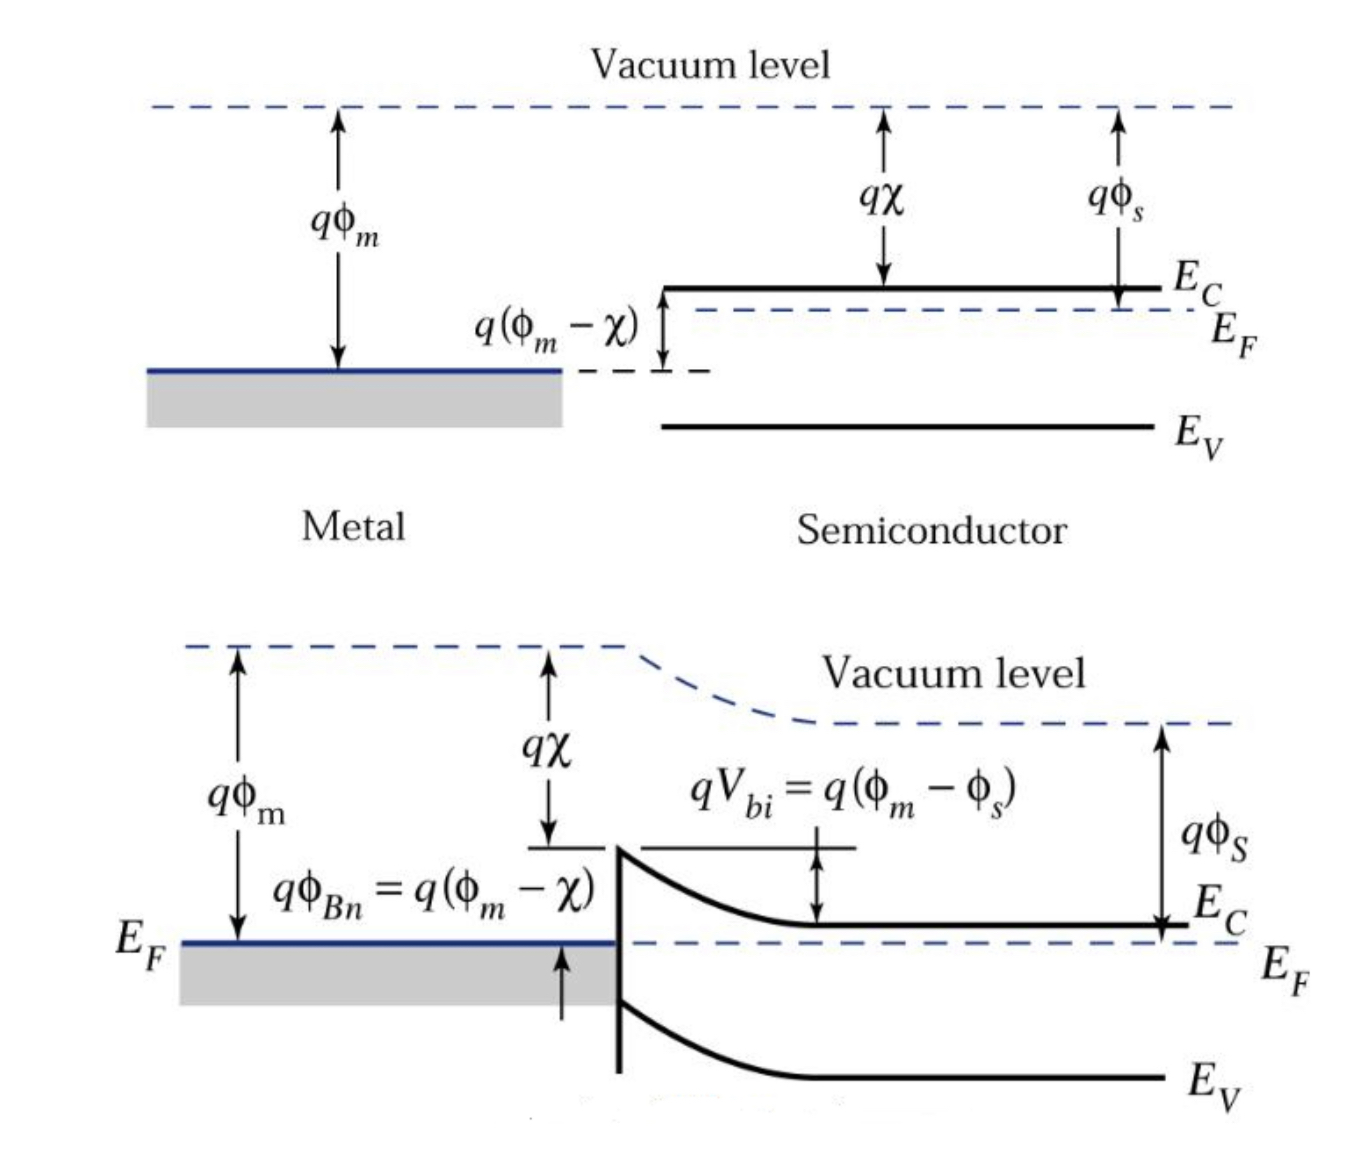
\includegraphics[width = 0.8\textwidth]{images/KM2/Schottky-Barriere.jpeg}
        \caption{Banddiagramm Schottky-Barriere}
        \label{fig:Schottky-Barriere}
    \end{figure}
    Die Banddiagramme sind in Abbildung \ref{fig:Schottky-Barriere} dargestellt. Im thermischen Gleichgewicht muss die Fermi-Energie konstant sein und die das Vakuumniveau muss stetig sein. Dadurch kommt es zu Bandverbiegungen der entsprechenden Energieniveaus\\
\end{addmargin}

\noindent\textbf{4. Wie kann man das gleichrichtende Verhalten von Metall-Halbleiter-Verbindungen umgehen?}\\
\begin{addmargin}[25pt]{0pt}
Dafür gibt es zwei Möglichkeiten, man kann entweder Metall und Halbleiter so wählen, dass $\phi_m \approx \chi$ ist, wodurch die Barriere zwischen Metall und Halbleiter sehr klein wird, oder man kann den Halbleiter stärker dotieren, das verringert zwar nicht die Höhe der Barriere allerdings wird ein durchtunneln durch diese deutlich wahrscheinlicher. $\chi$ ist die Elektronenaffinität des Halbleiters und $\phi_m$ die Austrittsarbeit des Metalls.   \\
\end{addmargin}

\subsubsection{Kurzfragen von Professor Pfleiderer}
\noindent\textbf{1. Worin unterscheiden sich Halbleiter von Isolatoren?}\\
\begin{addmargin}[25pt]{0pt}
Halbleiter sind Isolatoren mit kleinen Bandlücken, dadurch können Elektronen vom Valenzband in das Leitungsband übergehen. Bei der Temperatur $T=0$ sind alle Halbleiter Isolatoren. Bei höheren Temperaturen ist genug Energie im System damit manche Elektronen angeregt werden können. Typische Bandlücken für Halbleiter sind 0,75eV für Germanium; 1,1eV für Silizium und 1,4eV für Galliumarsenid. \\
\end{addmargin}

\noindent\textbf{2. Was sind direkte und indirekte Halbleiter?}\\
\begin{addmargin}[25pt]{0pt}
Die Bandlücke ist definiert als die Differenz der geringsten Energie des Leitungsbandes und der höchsten Energie des Valenzbandes. Bei direkten Halbleiter sind diese beiden Punkte im Banddiagramm direkt übereinander, also das VBM(valence band maximum) und das CBM (conduction band minimum) befinden sich am gleichen Ort im \textbf{k}-Raum. Bei indirekten Halbleitern sind das VBM und das CBM nicht übereinander und für einen Übergang wird ein Phonen vernichtet oder erschaffen. Beispiele für indirekte Halbleiter sind Silizium(Si) und Germanium(Ge). Ein Beispiel für direkte Halbleiter ist Galliumarsenid (GaAs).

\begin{figure}[h]
    \centering
    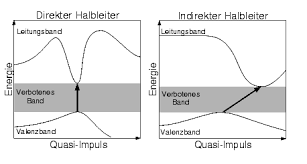
\includegraphics{images/KM2/direkt_indirekt_HL.png}
    \caption{Visualisierung von direkten und indirekten Halbleitern}
    \label{fig:direkte_indirekte_Halbleiter}
\end{figure}
\end{addmargin}

\noindent\textbf{3. Wie hängt die Bandlücke (intrinsischer Halbleiter) von T ab?}\\
\begin{addmargin}[25pt]{0pt}
Für tiefe Temperaturen ($T=0$\,K) ist die Bandlücke proportional zu $T^2$ und für höhere Temperaturen (im Bereich der Raumtemperatur) ist die Bandlücke proportional zu $T$. Dadurch ist die Bandlücke bei Raumtemperatur um 10\% geringer als bei $T=0$\,K. Die dafür verantwortlichen Effekte sind zum einen die thermische Expansion der Probe und dem damit verbunden größerem Abstand benachbarter Atome und zum anderen die Elektron-Phonon-Wechselwirkung.\\
\end{addmargin}

\noindent\textbf{4. Mit welcher Messgröße kann man direkte und indirekte Halbleiter unterscheiden?}\\
\begin{addmargin}[25pt]{0pt}
Man kann den Halbleiter mit elektromagnetischer Strahlung in einem großen Frequenzbereich bestrahlen und die Absorption messen. Ab einer Grenzenergie der Photonen reicht die Energie aus damit die Elektronen die Bandlücke überqueren können und man sieht einen starken Anstieg in der Absorption. Bei direkten Halbleitern steigt Absorption für noch höhere Energien nur noch minimal und kontinuierlich. Andererseits erkennt man in der Absorption von indirekten Halbleitern einen zweiten Absorptionssprung, dieser ist bei der Energie bei der für die Elektronen im indirekten Halbleiter auch ein direkter Übergang zum Leitungsband energetisch möglich wird. (Abbildung \ref{fig:Absorption_HL})\\
\begin{figure}[h]
    \centering
    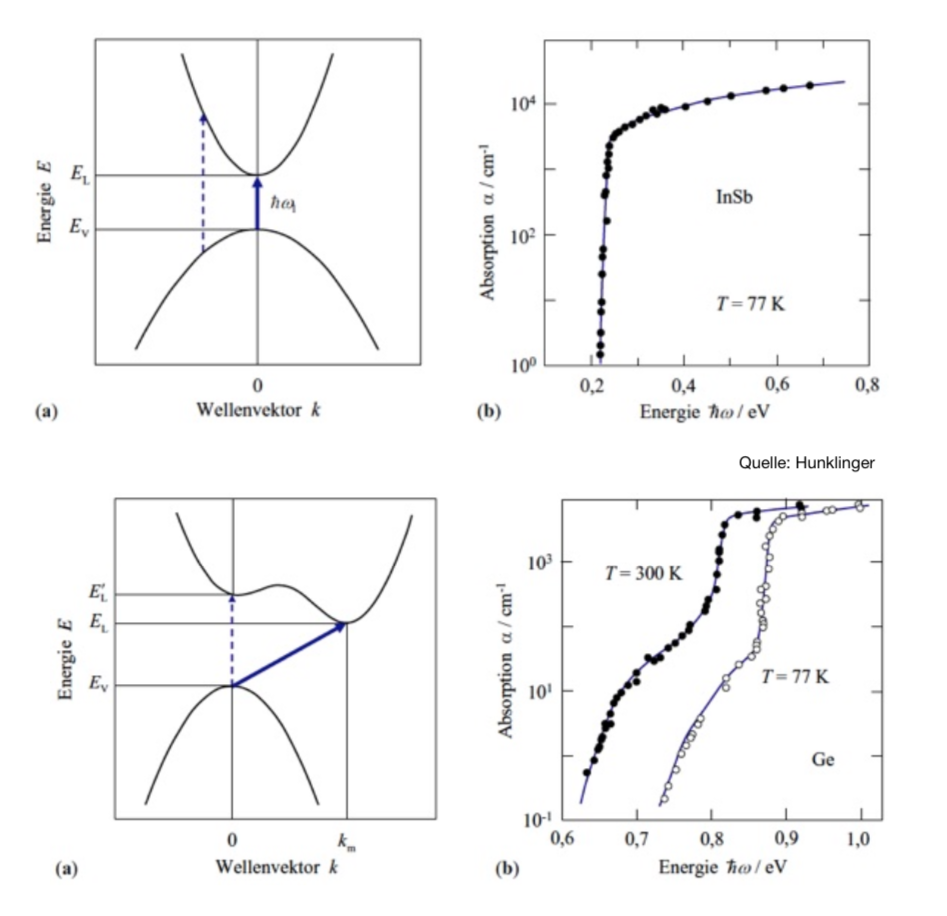
\includegraphics[scale = 0.8]{images/KM2/Absorption_HL.png}
    \caption{Absorptionsmessung für direkte und indirekte Halbleiter}
    \label{fig:Absorption_HL}
\end{figure}
\end{addmargin}

\noindent\textbf{5. Wie verhalten sich die effektiven Massen von intrinsischen Halbleitern?}\\
\begin{addmargin}[25pt]{0pt}
Im Allgemeinen ist die effektive Masse richtungsabhängig. Im Spezialfall der direkten Halbleiter ist der Tensor der effektiven Masse isotrop also richtungsunabhängig. Für den indirekten Halbleiter unterscheidet man zwischen longitudinaler und transversaler effektiver Masse, damit ist dieser Tensor nicht isotrop.  Der Tensor der effektiven Masse berechnet sich mit:
\begin{equation}\label{eq:effektive_Masse}
    m^*_{ij} = \hbar^2 \left(\frac{\partial^2 E}{\partial k_i\partial k_j}\right)^{-1}
\end{equation}
Bei der effektiven Masse ist häufig nur das CBM und VBM relevant da sich die Elektronen und Löcher fast immer in der Nähe dieser Punkte aufhalten.\\

\end{addmargin}

\noindent\textbf{6. Was versteht man unter Eigenleitung von intrinsischen Halbleitern?}\\
\begin{addmargin}[25pt]{0pt}
Die Eigenleitung ist der Teil der Leitfähigkeit, welcher nur durch Anregungen von Elektronen aus den Valenzband in das Leitungsband und Löchern aus dem Leitungsband in das Valenzband entsteht. Zusätzliche Leitfähigkeit wie Effekte durch Verunreinigungen oder Dotierung sind nicht Teil der Eigenleitung. \\
\end{addmargin}

\noindent\textbf{7. Wie hängen die Ladungsträgerkonzentrationen beim intrinsischen Halbleiter von der Temperatur ab?}\\
\begin{addmargin}[25pt]{0pt}
Für einen intrinsischen Halbleiter ist die Dichte der Löcher im Valenzband $p_i$ gleich der Dichte der Elektronen im Leitungsband $n_i$. Aus der Integration der Zustandsdichte über alle erlaubten Energien und unter Berücksichtigung der Fermi-Dirac-Statistik für Fermionen erhält man die Proportionalität:
\begin{equation}\label{eq:Ladungsträgerdichte_intrinsisch_Temperatur}
    n_i = p_i \propto k_BT^{\frac{3}{2}}e^{-\frac{E_g}{2k_bT}}
\end{equation}
Dabei ist $T$ die Temperatur, $k_B$ die Boltzmann-Konstante und $E_g$ die Bandlücke des Halbleiters.\\
\end{addmargin}

\noindent\textbf{8. Was versteht man unter dem Massenwirkungsgesetz?}\\
\begin{addmargin}[25pt]{0pt}
Das Massenwirkungsgesetz besagt, dass das Produkt aus der Elektronendichte im Leitungsband $n$ und der Löcherdichte im Valenzband $p$ eine Konstante ist, welche von den entsprechenden effektiven Massen der Löcher $m_h^*$ und der Elektronen $m_e^*$ abhängt:
\begin{equation}\label{eq:Massenwirkungsgesetz}
    n\cdot p = N_LN_Ve^{-\frac{E_g}{k_BT}}
\end{equation}
Die Konstanten sind ausgeschrieben:
\begin{align}
    N_L = 2\left(\frac{m_e^*k_BT}{2\pi\hbar^2}\right)^{\frac{3}{2}}\\
    N_V = 2\left(\frac{m_h^*k_BT}{2\pi\hbar^2}\right)^{\frac{3}{2}}
\end{align}\\
\end{addmargin}

\noindent\textbf{9. Wo befindet sich das Fermi Niveau beim intrinsischen Halbleiter?}\\
\begin{addmargin}[25pt]{0pt}
Die Fermi-Energie liegt für reine, nicht dotierte Halbleiter ungefähr in der Mitte der Bandlücke. Das ergibt aus Symmetriegründen Sinn, weil für jedes Elektron das vom Valenzband in das Leitungsband angeregt wird auch (ungefähr) ein Loch vom Leitungsband in das Valenzband springt. In der Realität weicht die Fermi-Energie etwas von der Mitte der Bandlücke ab da die Zustandsdichte von den Elektronen im Leitungsband nicht exakt gleich der Zustandsdichte der Löcher im Valenzband ist und somit auch deren Anzahl nach Gleichung \ref{eq:Besetzungszahl_e} und \ref{eq:Besetzungszahl_h} minimal voneinander abweicht:
\begin{align}\label{eq:Besetzungszahl_e}
n_e &= \int\limits_{E_L}^\infty D_L(E)f_{FD}(E,T)\si{d}E\\ \label{eq:Besetzungszahl_h} 
n_h &= \int\limits_{-\infty}^{E_V} D_V(E)\left(1-f_{FD}(E,T)\right)\si{d}E
\end{align}    
Dabei ist $D_V$ die Zustandsdichte der Löcher im Valenzband, $D_L$ die Zustandsdichte der Elektronen im Leitungsband, $E_V$ ist die Energie am VBM, $E_L$ die Energie am CBM und $f_{FD}(E,T) = \frac{1}{e^{\frac{E-E_F}{k_BT}}+1}$ die Fermi-Dirac-Verteilung. Unter Berücksichtigung dieser Zustandsdichten ergibt sich für die Fermi-Energie:
\begin{equation}
    E_{\si{F}} = \frac{E_{\si{V}} + E_{\si{L} }}{2} + \frac{k_BT}{2}\ln{\frac{N_V}{N_L}}
\end{equation}\\
\end{addmargin}

\noindent\textbf{10. Was sind typische Beispiele für dotierte kristalline Halbleiter?}\\
\begin{addmargin}[25pt]{0pt}
Man kann in einen kristallinen Halbleiter Dotieratome einbringen dadurch verändern sich die elektrischen Eigenschaften des Material. Man kann dabei entweder Donatoren oder Akzeptoren einbringen. Donatoren haben mehr Valenzelektronen als zu einer kovalenten Bindung benötigt werden und dadurch hat man mehr freie Elektronen im Kristall. Akzeptoren hingegen haben weniger Elektronen als für eine kovalente Bindung benötigt werden wodurch sie freie Löcher im Kristall erzeugen. Typischerweise nutzt man Phosphor, Arsen, Antimon oder Bismut als Donatoren und Bor, Aluminium, Gallium oder Indium als Akzeptoren. \\
\end{addmargin}

\noindent\textbf{11. Wie groß sind typische Ladungsträgerkonzentrationen beim intrinsischen und dotierten Halbleiter?}\\
\begin{addmargin}[25pt]{0pt}
Die Ladungsträgerkonzentration hängt sehr stark von der Art der Dotieratome und der Konzentration dieser ab. Dadurch kann man eine weite Bandbreite an Ladungsträgerkonzentrationen erreichen. Bei intrinsischen Halbleitern ist die Ladungsträgerkonzentration bei $\approx 10^{19} \frac{1}{\si{m}^3}$ für Germanium, $\approx 10^{16} \frac{1}{\si{m}^3}$ für Silizium und $\approx 10^{12} \frac{1}{\si{m}^3}$ für Gallium-Arsenid. Die besten dotierten Halbleiter von Gallium-Arsenid erreichen sogar $\approx 10^{22} \frac{1}{\si{m}^3}$. Dotierte Silizium -und Germaniumkristalle kommen beide auf $\approx 10^{19} \frac{1}{\si{m}^3}$. Man erkennt also dass sich Germanium sehr schlecht dotieren lässt wohingegen die Ladungsträgerdichte für Gallium-Arsenid um 10 Größenordnungen mit einer Dotierung erhöht werden kann.\\
\end{addmargin}

\noindent\textbf{12. Wie groß sind typische Energieskalen bei dotierten Halbleitern?}\\
\begin{addmargin}[25pt]{0pt}
Eine wichtige Kenngröße für Halbleiter ist die Bindungsenergie der Elektronen/Löcher an die Atome. Das ist die Energie die benötigt wird um ein Elektron vom Valenzband in das Leitungsband zu heben. Wir erwarten bei dotierten Halbleitern eine sehr geringe Bindungsenergie, da bei ihnen ein Loch oder Elektron zusätzlich vorhanden ist und somit dieses nur eine sehr schwache Bindung hat. Diese Vermutung wird von einer Messung bestätigt. Typische Bindungsenergien sind im Bereich von $10$ bis $100 \;\si{ meV}$ \\
\end{addmargin}

\noindent\textbf{13. Wie groß ist der effektive Bohr-Radius eines Dotieratoms?}\\
\begin{addmargin}[25pt]{0pt}
Analog dazu, dass Dotieratome kleine Bindungsenergien haben haben sie auch große effektive Bohr-Radien. Das ist auch intuitiv klar, da schwache Bindung einen großen Abstand zwischen den Bindungspartnern ermöglicht. Dotieratome haben einen effektiven Bohr-Radius der in etwa $50$ bis $100$-mal größer ist als der Bohr-Radius des Wasserstoffatoms.   \\
\end{addmargin}

\noindent\textbf{14. Was versteht man unter \glqq Kompensation\grqq \; bei dotierten Halbleitern?}\\
\begin{addmargin}[25pt]{0pt}
Halbleitermaterialien wie Silizium kann man nicht komplett rein herstellen, also wird es immer Fremdatome in einem Siliziumkristall geben. Dotiert man nun einen solchen Kristall, dann kann es zu Kompensation kommen wenn genauso viele Donatoren wie Akzeptoren in dem Kristall vorhanden sind. Das passiert zum Beispiel, wenn vor der Dotierung nur Donatoren als Fremdatome vorhanden waren und dann mit genauso vielen Akzeptoren dotiert wurde. Das Resultat der Kompensation ist, dass keine freien mehr in dem Kristall vorhanden sind.\\
\end{addmargin}

\noindent\textbf{15. Wie liegen die effektiven Energieniveaus beim dotierten Halbleiter?}\\
\begin{addmargin}[25pt]{0pt}
Bei dotierten Halbleitern entstehen zusätzliche Energieniveaus, dotiert man mit einem Donator so entsteht ein zusätzliches Energieniveau knapp unterhalb des Leitungsbandes und dotiert man mit einem Akzeptor entsteht ein zusätzliches Energieniveau knapp überhalb des Valenzbandes. Diese Niveaus sind in Abbildung \ref{fig:Energieniveaus_Halbleiter} gekennzeichnet.
\begin{figure}[h]
    \centering
    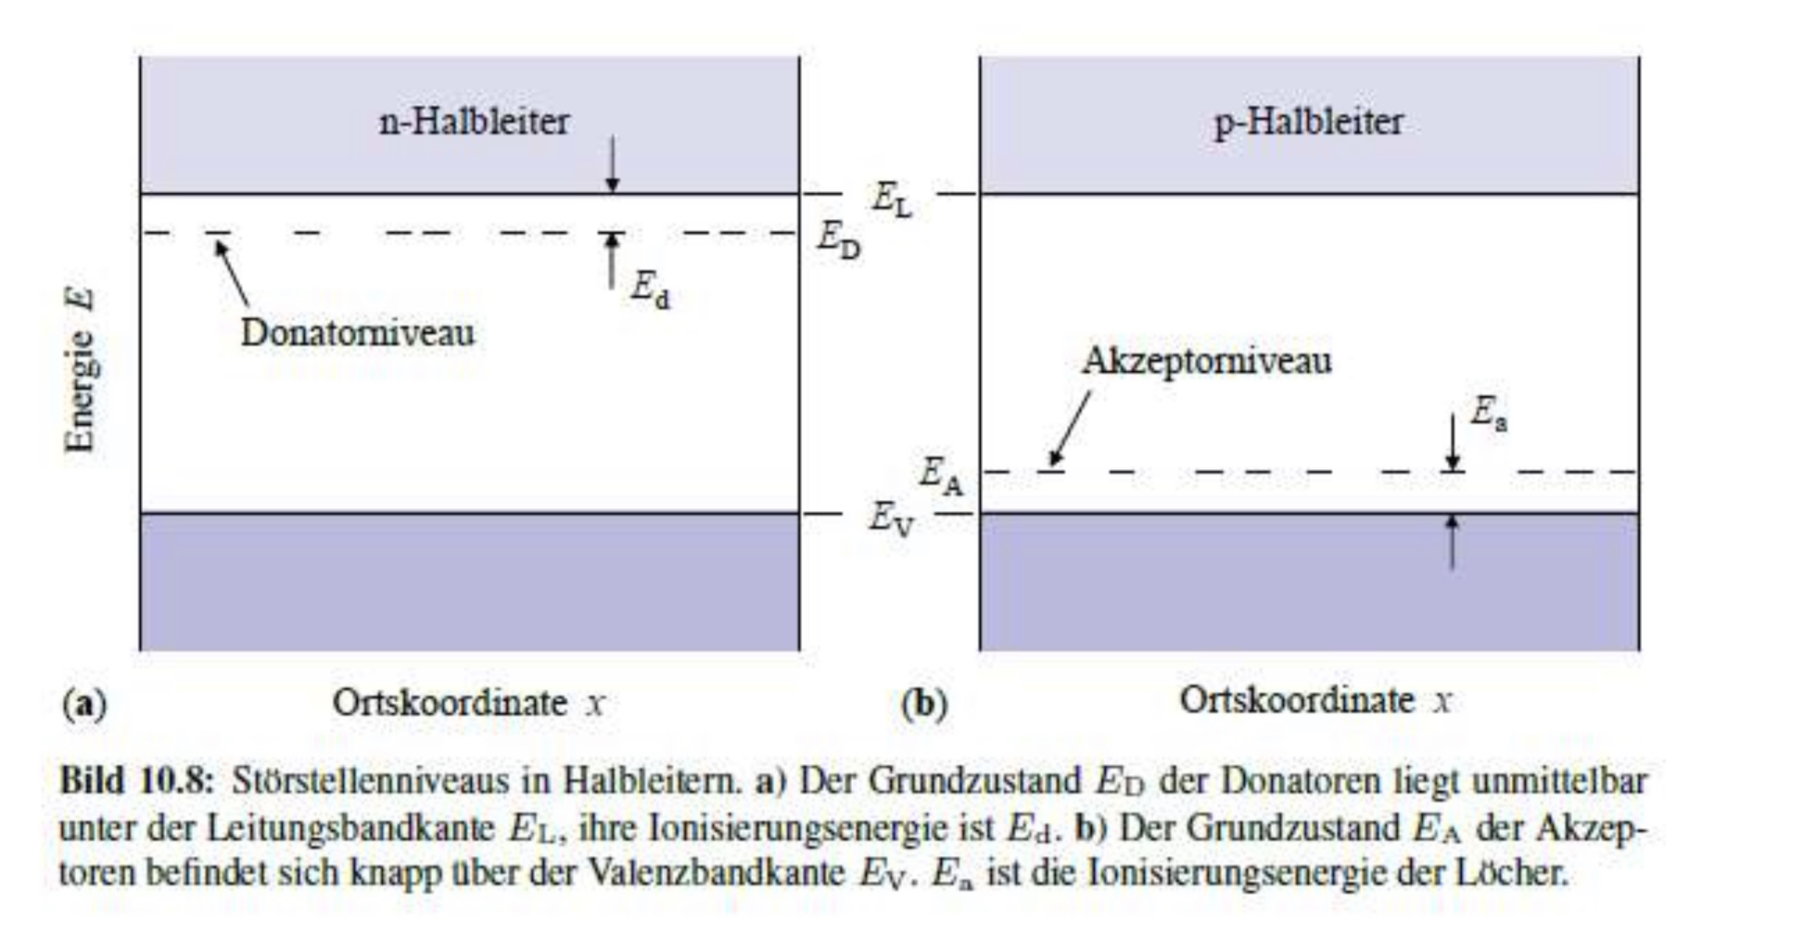
\includegraphics[width = 0.8\textwidth]{images/KM2/Donator_Akzeptorniveaus.jpeg}
    \caption{Darstellung der zusätzlichen Energieniveaus in dotierten Halbleitern}
    \label{fig:Energieniveaus_Halbleiter}
\end{figure}
Eine wichtige Konsequenz dieser zusätzlichen Niveaus ist, dass die Elektronen jetzt nicht mehr die gesamte Bandlücke überwinden müssen um auf ein höheres Niveau zu springen sondern nur noch von $E_V$ zum Akzeptorniveau $E_A$. Analog gilt das ganze für Löcher und das Donatorniveau $E_D$.
\end{addmargin}

\noindent\textbf{16. Was versteht man unter Kompensationsbereich, Störstellenreserve, Erschöpfungszustand und Eigenleitung und wie variiert jeweils die Elektronendichte mit T? }\\
\begin{addmargin}[25pt]{0pt}
In Abbildung \ref{fig:Elektronendichte_T_dotiert} kann man die Abhängigkeit der Elektronendichte von der Temperatur bei einem dotierten Halbleiter sehen, dieser Halbleiter hat einige Akzeptoren als Verunreinigungen in sich aber sehr viele Donatoren durch die Dotierung. In diesem Graphen gibt es 4 Bereiche, bei ganz niedrigen Temperaturen befindet sich der Kompensationsbereich, in diesem gibt es nur sehr wenige freie Ladungsträger und bei steigender Temperatur geben die vorhandenen Donatoren Elektronen ab, diese werden mit gleicher Wahrscheinlichkeit entweder von einem Akzeptor aufgenommen oder stehen als freie Elektronen zur Verfügung. Sobald alle Akzeptoren ein Elektron aufgenommen haben sind immernoch Donatoren verfügbar welche ihr zusätzliches Elektron noch nicht abgegeben haben, bei steigender Temperatur werden auch sie ihr Elektron abgeben und die Anzahl der freien Ladungsträger steigt nun doppelt so stark da abgegebenen Elektronen auch freie Ladungsträger sind. Diesen Bereich nennt man Störstellenreserve. Ab einer gewissen Temperatur haben alle Donatoren ihr Elektron abgegeben, die Elektronendichte bleibt in diesem Erschöpfungszustand für einen gewissen Temperaturbereich konstant. Bei sehr großen Temperaturen kommt es dann zur Eigenleitung, dabei werden dann vom Grundmaterial Ladungsträger direkt in das Leitungsband angelegt.\\
\begin{figure}[h]
    \centering
    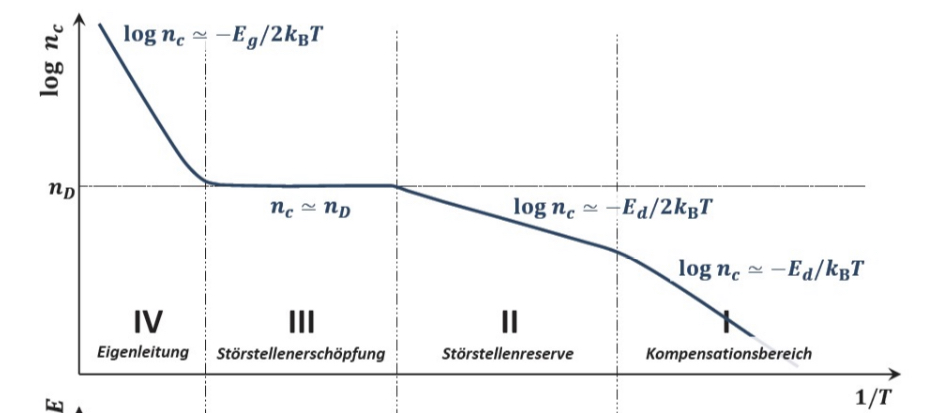
\includegraphics[width = 0.8\textwidth]{images/KM2/Elektronendichte_T_dotierteHL.jpeg}
    \caption{Verhalten der Elektronendichte in Abhängigkeit von der Temperatur bei einem n-Typ halbleiter}
    \label{fig:Elektronendichte_T_dotiert}
\end{figure}
\end{addmargin}

\noindent\textbf{17. Wie verändert sich die Lage des Fermi-Niveaus mit der Temperatur beim dotierten Halbleiter?}\\
\begin{addmargin}[25pt]{0pt}
Der Verlauf der Fermi-Energie in Abhängigkeit von der Temperatur ist in Abbildung \ref{fig:Fermi_Energie_dotiert_Temperatur} dargestellt. Für besonders große Temperaturen, im Bereich der Eigenleitung, befindet sich das Fermi-Niveau in der Mitte des Valenzbands und Leitungsbands, da der Beitrag durch die Elektronen dominiert wird, die vom Valenzband in das Leitungsband angeregt werden. Den Bereich der Störstellenreserve kann man analog beschreiben, allerdings kommen dort alle beteiligten Elektronen aus dem Donatorniveau und somit befindet sich die Fermi-Energie zwischen Donatorniveau und Leitungsband. Erhöht man von der Störstellenreserve die Temperatur werden im Bereich der Störstellenerschöpfung keine Elektronen mehr aus dem Donatorniveau kommen, dafür immer mehr intrinsisch Elektronen, angeregte aus dem Valenzband. Die Fermi-Energie sinkt also Richtung $\frac{E_g}{2}$. Zuletzt muss man noch den Bereich mit sehr kleinen Temperaturen betrachten, den Kompensationsbereich. In diesem Bereich werden, durch die vorhandenen Akzeptoren, nur die Hälfte aller vom Donator freigegebenen Elektronen auch in das Leitungsband angeregt, dadurch ist die Fermi-Energie genau das Donatorniveau.\\ 
\begin{figure}[h]
    \centering
    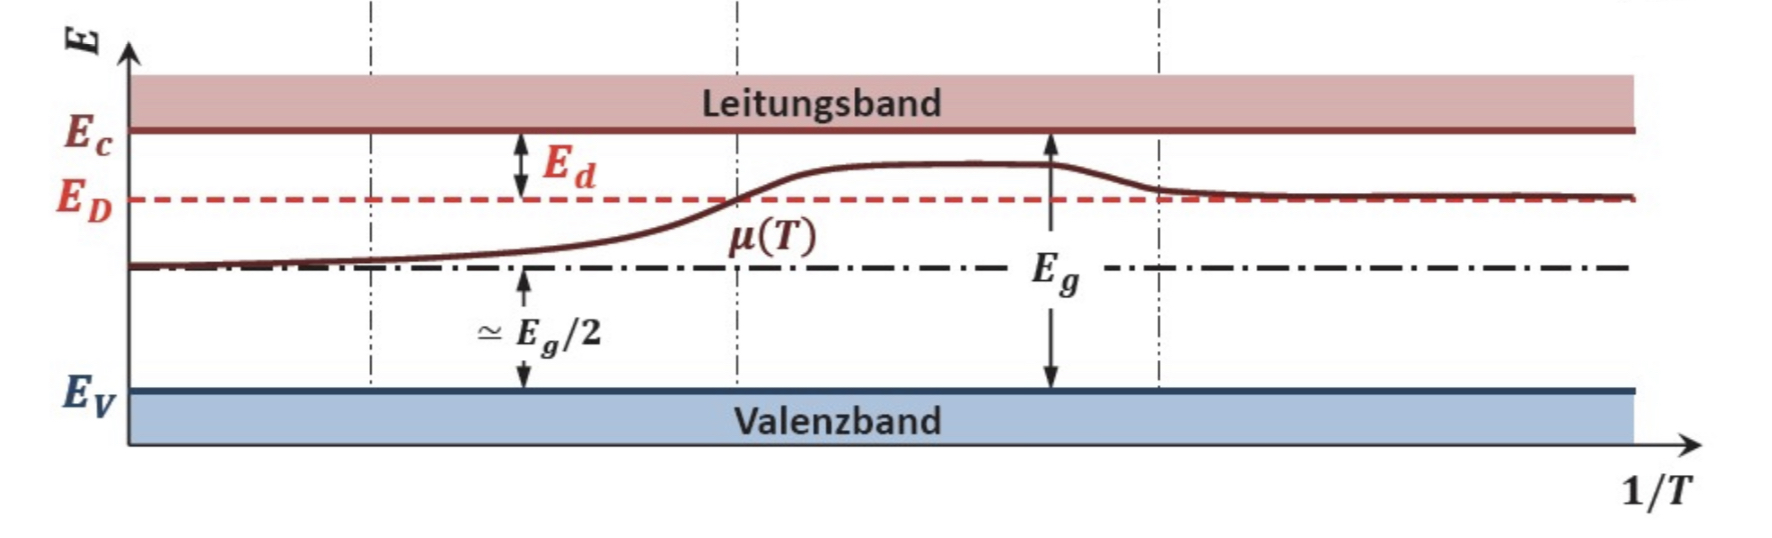
\includegraphics[width = \textwidth]{images/KM2/Fermi_Niveau_Temperatur_dotiert.jpeg}
    \caption{Die Lage des Fermi-Niveaus in den verschiedenen Temperaturbereichen Kompensationsbereich, Störstellenreserve, Störstellenerschöpfung und Eigenleitung für einen n-Typ Halbleiter}
    \label{fig:Fermi_Energie_dotiert_Temperatur}
\end{figure}
\end{addmargin}

\noindent\textbf{18. Wie verändert sich die Beweglichkeit und elektrische Leitfähigkeit mit T?}\\
\begin{addmargin}[25pt]{0pt}
Die Leitfähigkeit $\sigma_i$ hat sowohl einen Anteil von den Elektronen als auch von den Löchern. Sie lautet:
\begin{equation}\label{eq:leitfähigkeit}
    \sigma_i = \sigma_e + \sigma_h = n_i\mu_e e + p_i\mu_h e
\end{equation}
Dabei sind $n_i$ und $p_i$ die schon bekannte Elektronen- und Lochdichte und $\mu_e$ beziehungsweise $\mu_h$ die Beweglichkeiten der Elektronen und Löcher. Die Beweglichkeiten und die Ladungsträgerdichten haben jeweils eine Temperaturabhängigkeit. Die Beweglichkeiten berechnet man mit:
\begin{equation}\label{eq:beweglichkeit_definition}
    \mu_{e|h} = \frac{e\tau_{e|h}}{m^*_{e|h}}
\end{equation}
Dabei ist $\tau_{e|h}$ die temperaturabhängige Stoßzeit zwischen 2 Stößen eines Elektrons bzw. Lochs mit einem Defekt oder einem Phonon. Die Abhängigkeit der Beweglichkeit von der Temperatur ist in Abbildung \ref{fig:Beweglichkeit_Temperatur} dargestellt. Für niedrige Temperaturen dominiert der Anteil der geladenen Störstellen und für hohe Temperaturen der Anteil der Phononen. \\

\begin{figure}[h]
    \centering
    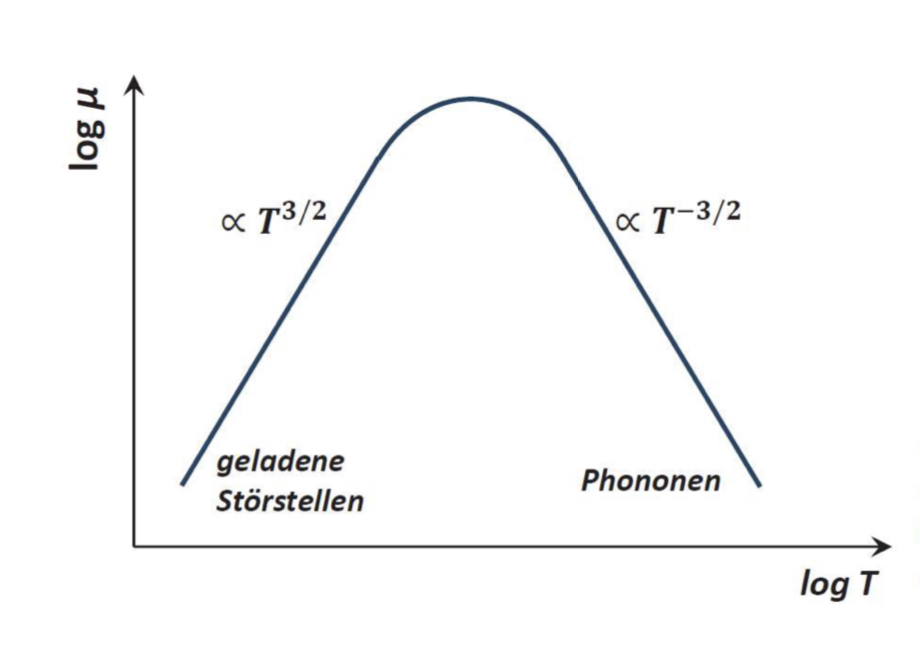
\includegraphics[width = \textwidth]{images/KM2/Beweglichkeit_Temperatur.jpeg}
    \caption{Die Abhängigkeit von der Beweglichkeit von der Temperatur}
    \label{fig:Beweglichkeit_Temperatur}
\end{figure}
\end{addmargin}

\noindent\textbf{19. Welche Rolle spielen Phononen für die Temperaturabhängigkeit der Leitfähigkeit?}\\
\begin{addmargin}[25pt]{0pt}
Phononen haben einen wesentlichen Einfluss auf die Stoßzeit von Elektronen beziehungsweise Löchern bei hohen Temperaturen (siehe Abbildung \ref{fig:Beweglichkeit_Temperatur}). Dadurch haben sie einen direkten Einfluss auf die Beweglichkeit und damit auf die Leitfähigkeit.\\
\end{addmargin}

\noindent\textbf{20. Was versteht man unter inhomogenen Halbleitern?}\\
\begin{addmargin}[25pt]{0pt}
Inhomogene Halbleiter haben keine konstante Dotierung beziehungsweise chemische Zusammensetzung. In dieser Art der Halbleiter können p-dotierte Bereiche direkt neben n-dotierten Bereichen liegen, das nennt man dann einen pn-Übergang. Inhomogene Halbleiter sind in der technischen Anwendung sehr bedeutend.\\
\end{addmargin}

\noindent\textbf{21. Was sind p- und n-Halbleiter?}\\
\begin{addmargin}[25pt]{0pt}
p-Halbleiter sind p-dotierte Halbleiter, also Halbleiter, welche mit Elektronenakzeptoren dotiert wurden. p-Halbleiter sind zum Beipsiel mit Bor, Gallium oder Indium dotiertes Silizium. n-Halbleiter wurden mit Donatoratomen dotiert. n-Halbleiter sind zum Beispiel mit Phosphor, Arsen, oder Antimon dotiertes Silizium.\\
\end{addmargin}

\noindent\textbf{22. Was sind Minoritäts- und Majoritätsladungsträger?}\\
\begin{addmargin}[25pt]{0pt}
Im n-Halbleiter hat man mehr Elektronen als Löcher und im p-Halbleiter ist es exakt anders herum. Die Majoritätsladungsträger sind dann die Art von Ladungsträger die mehr auftritt also Elektronen im n-Halbleiter und Löcher im p-Halbleiter. Die Minoritätsladungsträger sind jeweils die anderen also Löcher im n-Halbleiter und Elektronen im p-Halbleiter.\\
\end{addmargin}

\noindent\textbf{23. Wie verlaufen $E_L$ und $E_V$ beim pn-Übergang?}\\
\begin{addmargin}[25pt]{0pt}
Beim pn-Übergang befindet sich eine abrupte Grenze zwischen einem p-dotierten und einem n-dotierten Bereich (Abbildung \ref{fig:pn-transition}). Dadurch kommt es für die Elektronen und Löcher zu einem Konzentrationsgradienten, sodass die Elektronen nach links in Richtung p-dotierten Bereich diffundieren und die Löcher nach rechts in Richtung n-dotierten Bereich. An der Grenzfläche rekombinieren dann Elektronen mit Löchern, wodurch im p-dotierten Bereich dann Löcher und im n-dotierten Bereich Elektronen zur Ladungsneutralität fehlen. Dadurch ist der n-Bereich positiv und der p-Bereich negativ geladen wodurch sich ein Feld einstellt welches der Teilchendiffusion entgegenwirkt. Dieses entgegenwirkende elektrische Feld bewirkt eine Kraft auf die Löcher des n-Bereichs nach links und auf die Elektronen des p-Bereichs nach rechts. Wie in Abbildung \ref{fig:pn_transition_Raumladung} zu sehen bildet sich dadurch eine Raumladungszone um die Grenzfläche aus. Durch die Verschiebung und Rekombination der Ladungsträger werden auch das Valenz -und das Leitungsband verformt. Der Verlauf der Bänder am pn-Übergang ist in Abbildung \ref{fig:pn_transition_bandverlauf} dargestellt.\\

\begin{figure}[h]
    \centering
    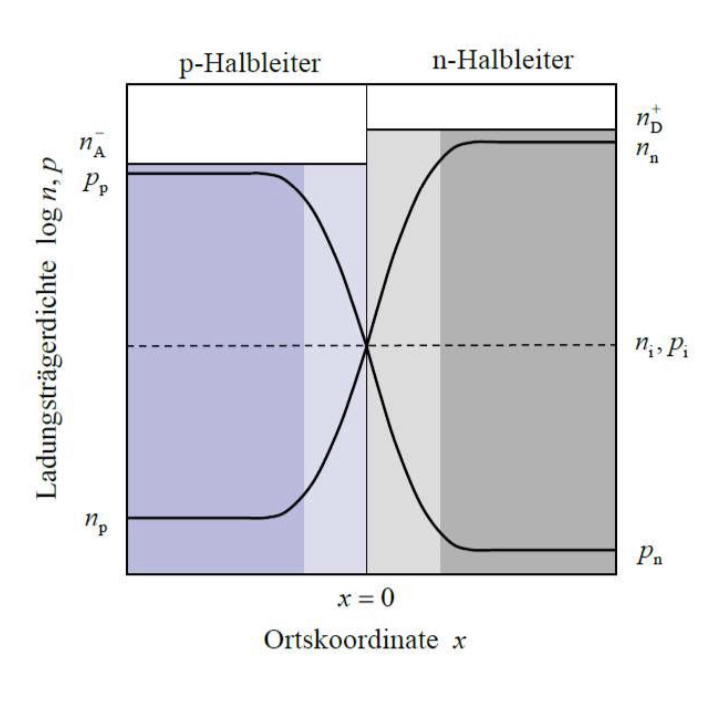
\includegraphics[width = 0.5\textwidth]{images/KM2/pn_transition.jpeg}
    \caption{Visualisierung der Ladungsträgerkonzentrationen beim pn-Üergang}
    \label{fig:pn-transition}
\end{figure}



\begin{figure}[h]
    \centering
    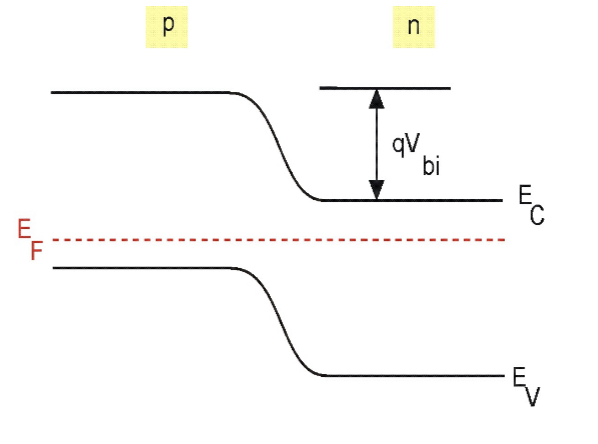
\includegraphics[width = 0.6\textwidth]{images/KM2/pn_transition_bandverlauf.jpeg}
    \caption{Verlauf des Valenzbandes und des Leitungsbandes am pn-Übergang}
    \label{fig:pn_transition_bandverlauf}
\end{figure}
\end{addmargin}
\newpage
\noindent\textbf{24. Was sind die Verarmung und Raumladungszone beim pn-Übergang?}\\
\begin{addmargin}[25pt]{0pt}
Durch die Rekombination von Löchern mit Elektronen sind im p-Bereich weniger Löcher und im n-Bereich weniger Elektronen frei verfügbar. Diese Verringerung an freien Laundgsträgern nennt man Verarmung. Die Raumladungszone ist der Bereich um die Grenzfläche, welcher nach dem Einstellen des Gleichgewichts aus Diffusionsstrom und Gegenfeld eine Nettoladung aufweist. Dieser ist in Abbildung \ref{fig:pn_transition_Raumladung} dargestellt. \\

\begin{figure}[h]
    \centering
    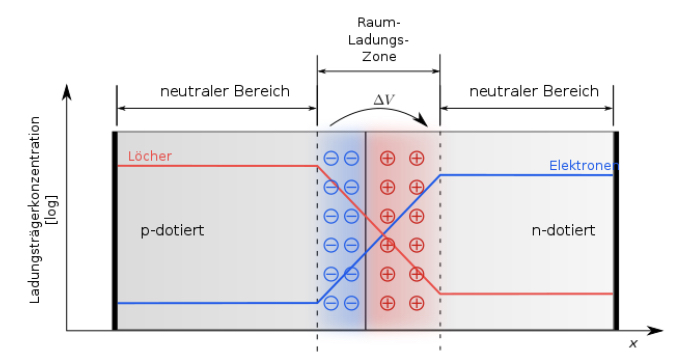
\includegraphics[width = 0.8\textwidth]{images/KM2/pn_transition_Raumladungszone.jpeg}
    \caption{Visualisierung der Raumladungszone beim pn-Übergang}
    \label{fig:pn_transition_Raumladung}
\end{figure}
\end{addmargin}

\noindent\textbf{25. Welche Annahmen werden beim Schottky-Modell des pn-Übergangs gemacht?}\\
\begin{addmargin}[25pt]{0pt}
Das Schottky-Modell nimmt eine scharfe Grenze der Raumladungszone an, also die Ladungsverteilung ist ein Rechteck. Außerdem muss gelten, dass die Gesamtladung der Raumladungszone null ist. Also muss gelten $en_Ad_p = en_Dd_n$, dabei ist $d_p$ die Breite der Raumladungszone von der Grenzfläche zum linken Rand, $d_n$ die Breite von der Grenzfläche zum rechten Rand und $n_A$ beziehungsweise $n_D$ sind die Ladungsträgerdichten im p-Bereich beziehungsweise im n-Bereich. Diesen Ansatz der konstanten, an der Grenze abbrechenden Ladungsverteilungen kann man nun in die Poisson-Gleichung:
\begin{equation}\label{eq:Poissono-Gleichung}
    \frac{\partial^2V(x)}{\partial x^2} = -\frac{\rho(x)}{\epsilon_r\epsilon_0}
\end{equation}
einsetzen und erhält unter Berücksichtigung der Bedingung $V(\infty) - V(-\infty) = V_D$ mit $eV_D = E_{gap}$ einen Ausdruck für die Breite der Raumladungszone:
\begin{equation}\label{eq:Breite_Raumladungszone}
    d_{n,p} = \sqrt{\frac{2\epsilon_r\epsilon_0V_D}{e} \frac{\frac{n_{A,D}}{n_{D,A}}}{n_A + n_D}}
\end{equation}\\
\end{addmargin}

\noindent\textbf{26. Was sind der Diffusionsstrom und der Feldstrom beim pn-Übergang?}\\
\begin{addmargin}[25pt]{0pt}
Der Diffusionsstrom ist der Strom der aufgrund des Konzentrationsgradienten zwischen n- und p-Halbleiter entsteht, er besteht aus den jeweiligen Majoritätsladungsträgern in dem entsprechenden Bereich. Durch die Rekombination an der Grenzfläche entsteht eine positive Nettoladung im n-Bereich und eine negative im p-Bereich, diese Ladungsbereiche rufen ein elektrisches Feld hervor, welches die jeweiligen Minoritätsladungsträger in den einzelnen Bereichen Richtung Grenzfläche verschiebt, diesen Strom aus Minoritätsladungsträgern nennt man Feldstrom. Im thermischen Gelichgewicht sind der Diffusionsstrom und der Feldstrom betragsgleich und entgegengesetzt gerichtet, so entsteht ein stationärer Zustand mit ausgeprägter Raumladungszone.\\
\end{addmargin}

\noindent\textbf{27. Wie verhält sich der pn-Übergang unter einer äußeren Spannung?}\\
\begin{addmargin}[25pt]{0pt}
Wir nehmen an, dass die gesamte Spannung über die Raumladungszone abfällt und der restliche Halbleiter feldfrei ist. Mit dieser Annahme kann man sich überlegen wie sich der pn-Übergang verhält wenn eine Spannung angelegt wird. Dabei muss man 2 Fälle unterscheiden. Im ersten Fall wird der Plus-Pol am p-Halbleiter angelegt und der Minus-Pol am n-Halbleiter, durch diesen Aufbau wird die Dicke der Raumladungszone verringert und es kann ein Strom fließen, das nennt man Durchlassrichtung. Der entgegengesetzte Fall erhöht die Dicke der Raumladungszone, wodurch kein Strom durch durch den pn-Übergang fließen kann. Das nennt man Sperrrichtung. \\
\end{addmargin}

\noindent\textbf{28. Was ist ein Zener-Durchbruch und was eine Zener-Diode?}\\
\begin{addmargin}[25pt]{0pt}
Eine Zener-Diode ist ein pn-Übergang, welcher darauf ausgelegt ist dauerhaft in Sperrrichtung betrieben zu werden. Legt man eine Spannung an dieses Bauteil an, so wird trotzdem kein Strom fließen. Es fließt erst ein Strom wenn die angelegte Spannung einen bestimmten Grenzwert überschreitet. Das geschieht, weil bei diesen hohen Feldern die Elektronen genügend Energie besitzen um durch die Raumladungszone durch zu tunneln. Diesen Durchruch nennt man Zener-Durchbruch.\\
\end{addmargin}

\noindent\textbf{29. Was versteht man unter einem Schottky-Kontakt?}\\
\begin{addmargin}[25pt]{0pt}
Ein Schottky-Kontakt ist ein Bauteil, welches aus einem dotierten Halbleiter und einem Metall besteht. Im Allgemeinen besitzen diese unterschiedlich hohe Fermi-Niveaus. Die Fermi-Niveaus gleichen sich dann an indem Ladungsträger über die Grenzfläche von Metall und Halbleiter diffundieren.\\
\end{addmargin}

\noindent\textbf{30. Was sind Halbleiterheterostrukturen?}\\
\begin{addmargin}[25pt]{0pt}
Halbleiterheterostrukturen sind im einfachsten Fall 2 aneinander gebrachte Halbleiter mit unterschiedlichen Valenzband- und Leitungsbandenergien. Dadurch entstehen Unstetigkeiten am Übergang. Ein Resultat daraus ist, dass im atomaren Bereich sehr hohe elektrische Felder auftreten können. In der Praxis werden diese Bauteile verwendet da sie eine sehr starke Verbesserung der Mobilitäten ermöglichen.\\
\end{addmargin}

\noindent\textbf{31. Was sind dotierungsmodulierte Kompositionsübergitter?}\\
\begin{addmargin}[25pt]{0pt}
Dotierungsmodulierte Kompositionsübergitter sind Verbindungen bei denen abwechselnd Schichten aus einem stark n-dotierten Halbleiter und einem intrinsischen Halbleiter verbaut sind. Der dotierte Halbleiter bildet eine Verarmungszone aus wodurch senkrecht zu den Grenzflächen die Bewegung stark eingeschränkt ist. Allerdings können sich Bloch-Wellen entlang der Grenzfläche sehr gut ausbreiten.  \\
\end{addmargin}

\noindent\textbf{32. Inwiefern beruht eine Solarzelle auf einem pn-Übergang?}\\
\begin{addmargin}[25pt]{0pt}
Eine Solarzelle besteht aus einem pn-Übergang. Ein einfallendes Photon kann, wenn seine Energie größer als die Energie der Bandlücke ist, ein Elektron-Loch Paar in der Raumladunszone erzeugen. Diese freien Ladungsträger werden im E-Feld der Raumladungszone getrennt, so entsteht ein zusätzlicher Strom in Richtung des Feldstroms. Dieser zusätzliche Strom kann über einen Verbraucher abgenommen werden. Allerdings wird ein Teil der erzeugten Ladungsträger wieder rekombinieren bevor er von einem Verbraucher abgegriffen werden kann.\\
\end{addmargin}

\noindent\textbf{33. Wie bestimmt man die maximale Leistung einer Solarzelle?}\\
\begin{addmargin}[25pt]{0pt}
Der Strom in einer Solarzelle hat mehrere Komponenten, eine Komponente durch den pn-Übergang und dessen Diffusions- und Feldstrom und eine Komponente $I_L$ in Richtung des Feldstroms. Der gesamte Strom ist dann:
\begin{equation}\label{eq:Kennlinie_Solarzelle}
    I = I_S\left(e^{\frac{eU}{k_BT}}-1\right) - I_L
\end{equation}
dieser Strom gegen die anliegende Spannung ist in Abbildung \ref{fig:Solarzelle} gezeigt. Die maximale Leistung $P_m$ ist das größte Rechteck was unter diese Kurve passt. Man kann in Abbildung \ref{fig:Solarzelle} auch sehr gut sehen, dass ohne $I_L$ also den Beitrag aus der Photoneneinstrahlung auch keine Leistung umgesetzt werden kann, weil die Kennlinie dann durch den Koordinatenursprung geht. 
\begin{figure}[h]
    \centering
    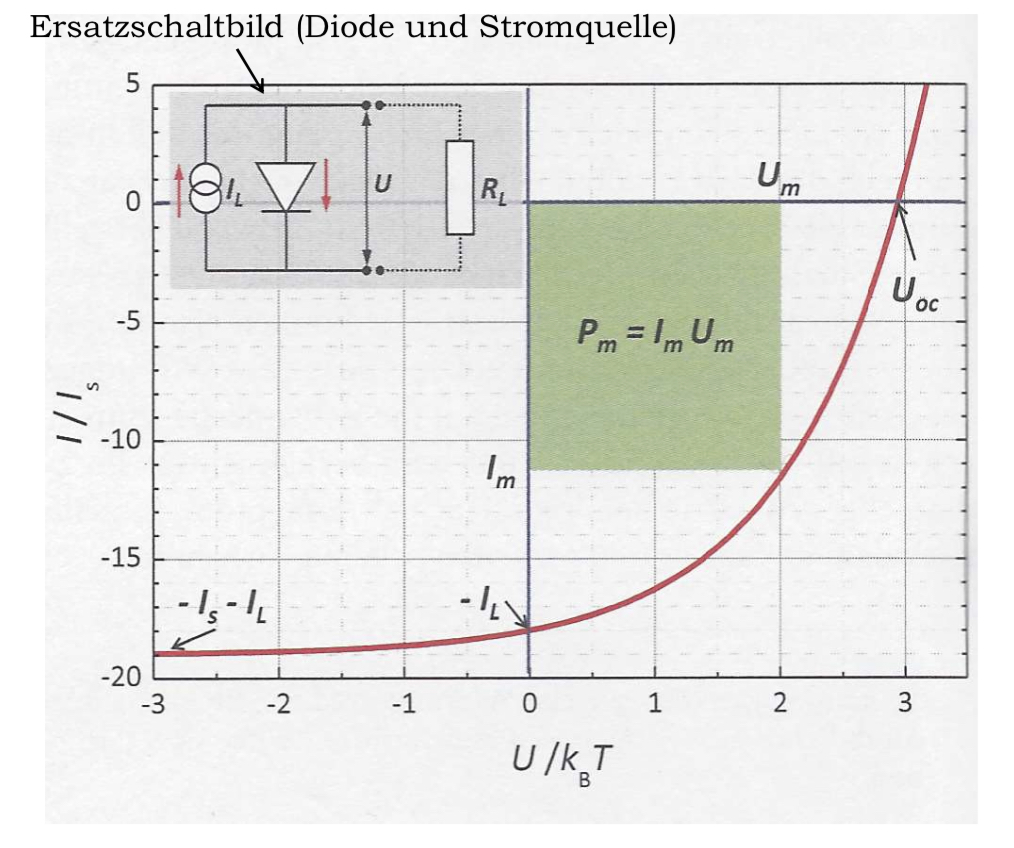
\includegraphics[width = 0.8\textwidth]{images/KM2/Solarzelle.jpeg}
    \caption{Kennlinie einer Solarzelle inklusive Ersatzschaltbild}
    \label{fig:Solarzelle}
\end{figure}
\end{addmargin}

\noindent\textbf{34. Was ist eine Photodiode und wie funktionieren CCD-Sensoren?}\\
\begin{addmargin}[25pt]{0pt}
Eine Photodiode funktioniert prinzipiell wie eine Solarzelle allerdings ist sie deutlich kleiner und wird nicht zur Stromerzeugung sondern zum Nachweis von Licht beispielsweise in Laboren verwendet.\\ 
CCD-Sensoren (charge coupled device) sind eine Matrixanordnung von Photodioden mit denen man nicht nur Licht nachweisen kann sondern dieses auch besser räumlich lokalisieren kann. CCD-Sensoren werden häufig in der Fotografie oder Videotechnik aber auch in Laboren verwendet.
\end{addmargin}

\noindent\textbf{35. Wie funktionieren Leuchtdioden?}\\
\begin{addmargin}[25pt]{0pt}
Leuchtdioden bestehen ebenfalls aus einem pn-Übergang, bei ihnen wird durch ein äußeres elektrisches Feld gezielt eine Rekombination von Elektron mit Loch hervorgerufen, also quasi der umgekehrte Effekt der bei der Solarzelle ausgenutzt wird. Durch diese Rekombination wird ein Photon abgegeben wodurch man aus elektrischem Strom Licht produziert hat. Die Wellenlänge der Photons hängt von der Dotierung, genauer der Bandlücke, der Leuchtdiode ab. \\
\end{addmargin}

\noindent\textbf{36. Was ist ein \glqq transfer resistor\grqq ?}\\
\begin{addmargin}[25pt]{0pt}
Ein \glqq transfer resistor\grqq ist besser bekannt unter dem Namen Transistor. Es gibt pnp- und npn-Transistoren, die sind aus 2 p-dotierten und einem n-dotierten Halbleiter aufgebaut bzw. 2 n-dotierten und einem p-dotierten. Dadurch bilden sich 2 Raumladungszonen aus, diese sind in Abbildung \ref{fig:Transistor}a grau dargestellt. Im Stromkreis wird der pn-Übergang von Emitter zu Basis in der Durchlassrichtung betrieben und der von Kollektor und Basis in der Sperrrichtung. Man kann bei einem Transistor den Stromfluss von Emitter zu Kollektor steuern in dem man einen Basisstrom $I_b$ anlegt. Je nach der Stärke des Basisstroms kann der Stromfluss entweder komplett unterdrückt oder um einen großen Faktor verstärkt werden.\\
\begin{figure}[h]
    \centering
    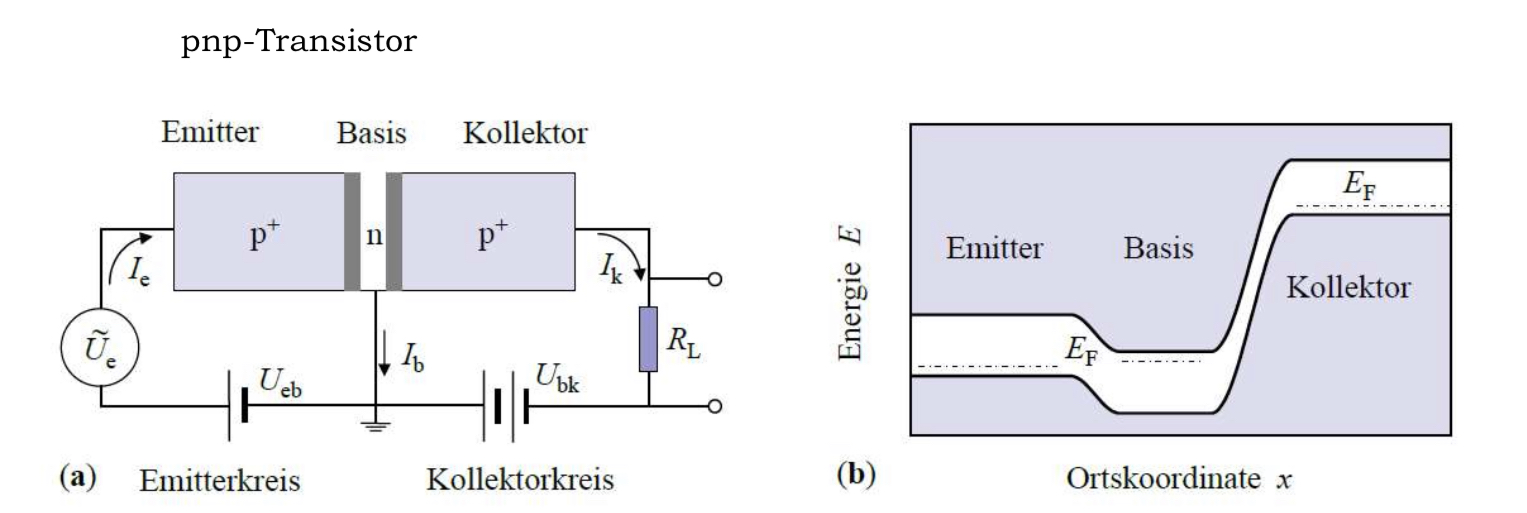
\includegraphics[width = \textwidth]{images/KM2/Transistor.jpeg}
    \caption{(a) schematische Darstellung eines pnp-Transistors in einem Stromkreis (b) Bandschema in einem Transistor}
    \label{fig:Transistor}
\end{figure}
\end{addmargin}

\noindent\textbf{37. Was kann man mit einem pnp-Übergang machen? (Funktionsweise)}\\
\begin{addmargin}[25pt]{0pt}
Mit einem pnp-Übergang kann man einen Stromfluss steuern und verstärken. Der Strom von Emitter zu Kollektor fließt dabei nur wenn auch ein Basisstrom fließt, also eine Spannung zwischen Emitter und Basis anliegt.\\
\end{addmargin}

\noindent\textbf{38. Was ist ein MOSFET und wie funktioniert er?}\\
\begin{addmargin}[25pt]{0pt}
MOSFET steht für Metal-Oxide-Semiconductor Field Effect Transistor. Ein MOSFET hat einen ähnlichen Effekt wie ein pnp- oder npn-Transistor. Wie in Abbildung \ref{fig:MOSFET} dargestellt kann man durch Anlegen einer Spannung $V_g$ an das Gate einen Kanal zwischen Source und Drain erzeugen durch welchen Stromfluss möglich wird. Durch die Stärke der Spannung $V_g$ kann man die Dicke des Kanals und somit die Stärke des Stromflusses bestimmen.\\ 
\begin{figure}[h]
    \centering
    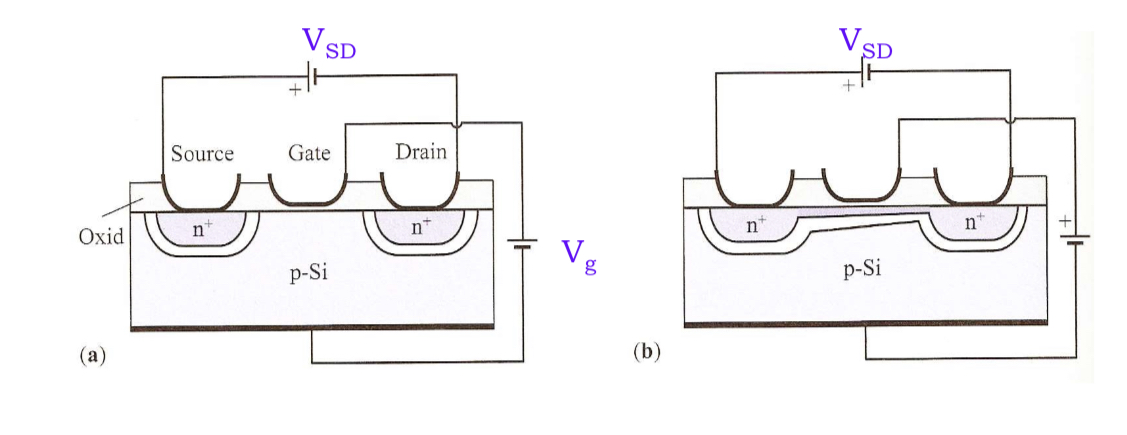
\includegraphics[width = \textwidth]{images/KM2/MOSFET.jpeg}
    \caption{Funktion eines MOSFETs}
    \label{fig:MOSFET}
\end{figure}
\end{addmargin}

\noindent\textbf{39. Wie funktionieren Halbleiterlaser?}\\
\begin{addmargin}[25pt]{0pt}
Ein Halbleiterlaser funktioniert im Prinzip ähnlich wie eine Photodiode nur mit deutlich höheren Intensitäten des Lichts. Diese werden unter Anderem dadurch erreicht, dass reflektierende Schichten die emittierten Photonen zurück in den Laser bringen und dadurch noch deutlich mehr Rekombinationen und schließlich stimulierte Emissionen von Photonen stattfinden können.\\
\end{addmargin}

\subsection{Magnetismus}

\noindent\textbf{1. Welcher Zusammenhang besteht zwischen magnetischem Moment und Drehimpuls?}\\
\begin{addmargin}[25pt]{0pt}
Das magnetische Moment $\vec{\mu}$ ist proportional zum Drehimpuls, dieser ist entweder $\Vec{L}$, $\Vec{S}$ oder $\Vec{J}$. Die Proportionalitätskonstante ist das gyromagnetische Verhältnis $\gamma$ multipliziert mit dem g-Faktor für die Art des Drehimpulses, dieser ist $g_l = 1$, $g_s \approx 2$ und $g_j$ der Landé-Faktor:
\begin{equation}\label{eq:Landé-Faktor}
    g_j = 1 + \frac{j(j+1) + s(s+1) - l(l+1)}{2j(j+1)}
\end{equation}
Das gyromagnetische Verhältnis ist eine Konstante die für das betrachtete Teilchen charakteristisch ist, dieses Verhältnis ist gegeben als:
\begin{equation}\label{eq:gyromagnetisches Verhältnis}
    \gamma = \frac{q}{2m}
\end{equation}
Also ergibt sich für das magnetische Moment für Elektronen $\Vec{\mu}_l$ (Hier beispielhaft für $\Vec{L}$ funktioniert aber analog für $\Vec{S}$ und $\Vec{J}$):
\begin{equation}\label{eq:magnetisches_Moment_Drehimpuls}
    \Vec{\mu}_l = \frac{-e}{2m_e}g_l\Vec{L}
\end{equation}
Durch die Quantisierung des Drehimpulses kann man den Betrag von $\vec{\mu}_l$ finden indem man $|\Vec{L}| = \hbar\sqrt{l(l+1)}$ verwendet:
\begin{equation}\label{eq:Betrag_magnetisches_Moment_Drehimpuls}
    |\Vec{\mu}_l| = \frac{e\hbar}{2m_e}g_l\;\sqrt{l(l+1)} = \mu_B\cdot g_l \cdot\sqrt{l(l+1)}
\end{equation}
Dabei ist $\mu_B = 9,274\cdot 10^{-24} \frac{\si{J}}{\si{T}}$ das \textit{Bohr'sche Magneton}.\\

\end{addmargin}

\noindent\textbf{2. Was ist der Einstein-deHaas-Effekt?}\\
\begin{addmargin}[25pt]{0pt}
Der Einstein-deHaas-Effekt zeigt den Zusammenhang zwischen Magnetimus und Drehimpuls im makroskopischen Bereich. Für dieses Experiment wird ein magnetisierbarer Stab an einen Faden gehangen. Der Stab befindet sich in einer Spule (siehe Abbildung \ref{fig:Einstein_deHaas}), wenn an die Enden der Spule ein Strom angelegt wird baut sich ein, zur Stabachse paralleles, Magnetfeld auf. Durch dieses Magnetfeld richten sich die Spins im Stab aus und dieser ist magnetisiert. Der Stab wird sich dann anfangen um seine Achse zu drehen, das kommt aus der Drehimpulserhaltung. Vor dem Einschalten des B-Feldes war der Gesamtdrehimpuls null und im atomaren die Spins ungeordnet, nach Einschalten des B-Feldes haben sich die Spins ausgerichtet und damit zeigt der Drehimpuls jedes Atoms in die selbe Richtung, aus der Drehimpulserhaltung folgt nun dass sich der Stab makroskopisch anfangen muss zu drehen.\\
\begin{figure}[h]
    \centering
    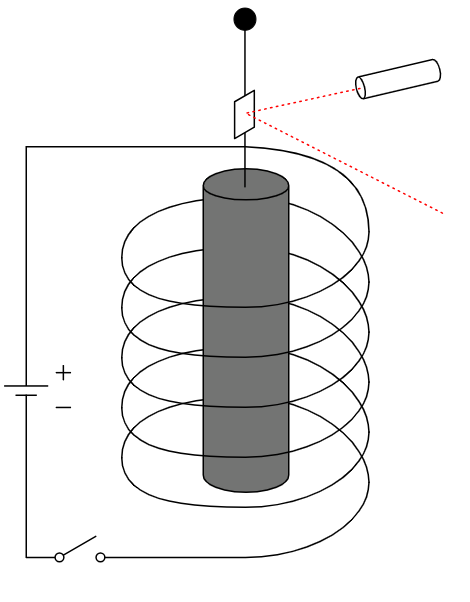
\includegraphics[width = 0.5\textwidth]{images/KM2/Einstein_deHaas.png}
    \caption{Der Versuchsaufbau des Einstein-deHaas-Effekts}
    \label{fig:Einstein_deHaas}
\end{figure}
\end{addmargin}
\vspace{5cm}
\noindent\textbf{3. Was ist die Larmor Präzession und die Larmor-Frequenz?}\\
\begin{addmargin}[25pt]{0pt}
Befindet sich ein Teilchen mit magnetischem Moment $\vec{\mu}$ in einem äußeren Magnetfeld $\Vec{B}$ so erfährt sein Drehimpuls eine Änderung aufgrund des Drehmoments $\Vec{M} = \Vec{\mu} \times \Vec{B}$. Eingesetzt in die Bewegungsgleichungen findet man: 
\begin{equation}\label{eq:Bewegungsgleichung_Larmor}
    \frac{\si{d}\vec{\mu}}{\si{d}t} = \gamma \Vec{\mu} \times \Vec{B}
\end{equation}
Daraus sieht man, dass die Änderung des magnetischen Moments senkrecht auf $\Vec{\mu}$ und $\Vec{B}$ steht, also das magnetische Moment präzediert um das äußere Magnetfeld. Die Frequenz dieser Larmor-Präzession nennt man Larmor-Frequenz:
\begin{equation}\label{eq:Larmor_Frequenz}
    \omega_L = \frac{eB}{2m_e}
\end{equation}
\end{addmargin}

\noindent\textbf{4. Wie hängen Magnetisierung und magnetisches Moment zusammen?}\\
\begin{addmargin}[25pt]{0pt}
Jedes Atom trägt in einem Festkörper ein magnetisches Moment. Dadurch hat der Festkörper im gesamten auch ein magnetisches Verhalten, dieses wird durch die Magnetisierung dargestellt. Die Magentisierung $\Vec{M}$ ist dabei ein Maß für die Menge an atomarem magnetischem Moment pro Volumen. Sie ist ein glattes Vektorfeld und wird berechnet mit:
\begin{equation}\label{eq:Definition_Magnetisierung}
    \Vec{M} = \frac{\partial \Vec{\mu}}{\partial V}
\end{equation}

\end{addmargin}

\noindent\textbf{5. Was sind Entmagnetisierungsfelder und Entmagnetisierungsfaktoren?}\\
\begin{addmargin}[25pt]{0pt}
Legt man ein äußeres Magnetfeld $\vec{B}_a$, $\Vec{H}_a$ an ein Material an, so wird aufgrund der Interaktion des äußeren Magnetfeldes mit den Atomen des Körpers das Magnetfeld im Körperinneren $\vec{B}_i$, $\Vec{H}_i$ ungleich dem von außen angelegten sein. Mit der Magnetisierung $\Vec{M}$ ergibt sich dann:
\begin{align}
    \Vec{H}_i &= \Vec{H}_a - N\cdot\Vec{M}\\
    \Vec{B}_i &= \Vec{B}_a + \mu_0 (1-N)\Vec{M}
\end{align}
In diesen Gleichungen nennt man $\Vec{H}_d = N\cdot\Vec{M}$ das Entmagnetisierungsfeld und $N$ den Entmagnetisierungsfaktor, dieser hängt dabei von der Geometrie des Körpers ab, für eine Kugel gilt zum Beispiel $N = \frac{1}{3}$.\\ 
\end{addmargin}

\noindent\textbf{6. Was besagt das Bohr-van-Leeuwen-Theorem?}\\
\begin{addmargin}[25pt]{0pt}
Das Bohr-van-Leeuwen-Theorem besagt, dass unter der Annahme von klassischen, nicht-wechselwirkenden Elektronen im Magnetfeld die Magnetisierung des Festkörpers exakt verschwindet. Das bedeutet, dass Magnetismus nicht mit der klassischen Physik erklärt werden kann sondern eine quantenmechanische Beschreibung der Systeme notwendig ist. In der Herleitung dieses Sachverhaltes stellt man die kanonische Zustandssumme basierend auf dem klassischen Hamilton-Operator auf. Man stellt fest, dass diese nicht mehr vom magnetischen Feld abhängt und somit die Magnetisierung, welche die Ableitung der freien Energie nach dem B-Feld ist, null sein muss. Die freie Energie ist proportional zum Logarithmus der Zustandssumme.  \\
\end{addmargin}

\noindent\textbf{7. Was sind \glqq skipping orbits\grqq ?}\\
\begin{addmargin}[25pt]{0pt}
Liegt ein Magnetfeld an einer Probe an, so bewegen sich nach klassischer Erwartung die Elektronen in der Probe auf Kreisbahnen. Dabei tritt ein Problem auf: Elektronen, welche sich nah am Rand der Probe befinden, müssten auf ihrer Kreisbahn den Körper verlassen und das ist nicht möglich. Diese Elektronen werden beim Auftreffen auf den Rand der Probe reflektiert und bewegen sich anschließend weiter auf einer Kreisbahn, da sie keine komplette Kreisbewegung vollführen sondern diese immer unterbrochen und neu angesetzt wird nennt man ihre Bewegung \glqq skipping orbits\grqq  \\
\end{addmargin}

\noindent\textbf{8. Wodurch entstehen die diamagnetische und paramagnetische Suszeptibilität isolierter magnetischer Momente?}\\
\begin{addmargin}[25pt]{0pt}
Paramagnetismus tritt nur in Materialien auf, welche ungepaarte Atome besitzen und ein magnetisches Moment besitzen. Die Elementarmagnete der Probe besitzen keine Ausrichtung ohne äußeres Feld. Legt man ein magnetisches äußeres Feld an, so richten sich  die Elementarmagnete bevorzugt mit der Richtung der Feldlinien aus. Für Paramagneten ist die Suszeptibilität $\chi >0$. Diamagnetismus entsteht in allen Materialien, allerdings ist der Effekt des Diamagnetismus so schwach, dass er nur relevant wird in Materialien die weder paramagnetisch noch ferromagnetisch sind. Für die diamagnetische Suszeptibilität gilt $\chi <0$. Diamagnete haben ebenso nur eine Ausrichtung der Elementarmagnete durch ein äußeres magnetisches Feld, bei ihnen richten sich die Elementarmagnete jedoch antiparallel zum äußeren B-Feld aus.\\
\end{addmargin}

\noindent\textbf{9. Wie hängen Diamagnetismus und Kernladungszahl zusammen?}\\
\begin{addmargin}[25pt]{0pt}
Diamagnetismus tretet nur in Isolatoren mit vollbestezten Elektronen auf. Die magnetische Suszeptibilität ist proportional zu der Anzahl der Elektronen in der äußersten Schale. Somit erhält man auch eine Abhängigkeit von der Kernladungszahl, da diese die Elektronenanzahl bestimmt.
\begin{equation}
    \chi_{dia} \approx -\mu_{0}\frac{e^2}{6m}\frac{N}{V}Z_{a}r^2_{a}
\end{equation}\\
\end{addmargin}

\noindent\textbf{10. Was beschreibt die Langevin-Gleichung?}\\
\begin{addmargin}[25pt]{0pt}
Die Langevin-Gleichung (\ref{eq:Langevin}) beschreibt das Verhältnis zwischen Magnetisierung und Sättigungsmagnetisierung von Paramagneten. Dieses Verhältnis entspricht der Anzahl der ausgerichteten magnetischen Momente. Für die Herleitung dieser Gleichung wurde angenommen, dass sich alle magnetischen Momente mit einem beliebigen Winkel ausrichten können (also klassische Betrachtung). Die Langevin-Gleichung ist in guter Nährung für große Quantenzahlen gültig.
\begin{equation}
    \frac{M}{M_{s}} = \frac{<\mu_{z}>}{\mu} = \coth{\frac{\mu B}{k_{B}T}} - \frac{k_{B}T}{\mu B} \equiv \mathcal{L} \left(\frac{\mu B}{k_{B}T}\right)
    \label{eq:Langevin}
\end{equation}
\begin{figure}
    \centering
    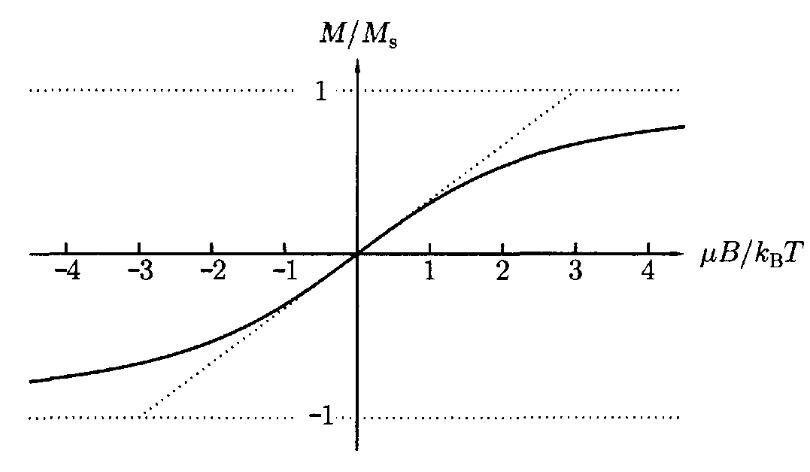
\includegraphics[scale=0.5]{images/KM2/Langevin-Velauf.png}
    \caption{Magnetisierung bei Paramagneten mit Langevin-Gleichung}
    \label{fig:Magnetisierung-Paramag}
\end{figure}\\
\end{addmargin}

\noindent\textbf{11. Was beschreibt die Brillouin Funktion?}\\
\begin{addmargin}[25pt]{0pt}
Die Briullin-Funktion (\ref{eq:Briullin-Fkt}) ist das quantenmechanische Analogon zur Langevin-Gleichung. Die Voraussetzung dieser Gleichung ist, dass der Gesamtdrehimpuls $J>1/2$ ist. Es wurde die Abkürzung $y=\frac{g_{j}\mu_{B}B_{ext}}{k_{B}T}J$ verwendet. In Abbildung (\ref{fig:Briullin-Verlauf}) sieht man den Unterschied zwischen der Briullin-Funktion und Langevin-Funktion.  
\begin{equation}
    \frac{M}{M_{s}} = \mathcal{B}_{J}(y) = \frac{2J+1}{2J}\coth{\frac{2J+1}{2J}y} -\frac{1}{2J} \coth{\frac{1}{2J}y}
    \label{eq:Briullin-Fkt}
\end{equation}
\begin{figure}
    \centering
    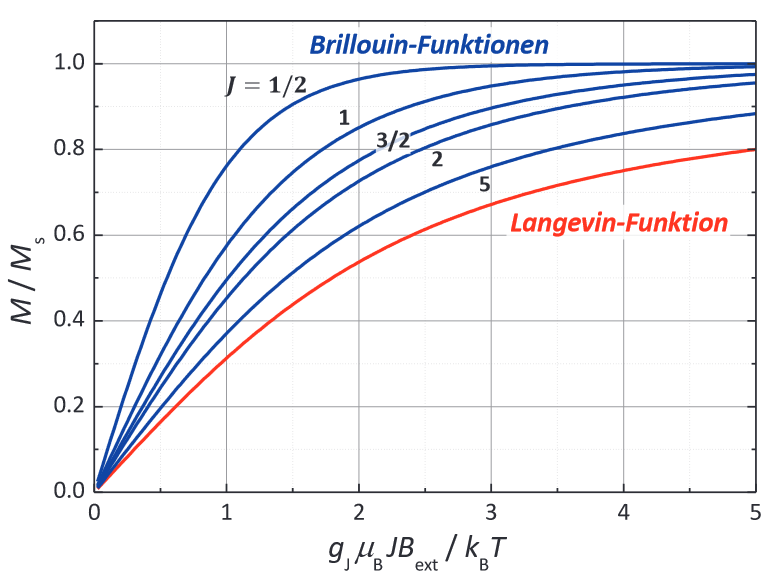
\includegraphics[scale=0.5]{images/KM2/Briullin-Verlauf.png}
    \caption{vergleich zwischen Briullin- und Langevin-Verlauf.}
    \label{fig:Briullin-Verlauf}
\end{figure}\\
\end{addmargin}

\noindent\textbf{12. Was versteht man unter Curie-Verhalten?}\\
\begin{addmargin}[25pt]{0pt}
Das Curie-Gesetz besagt, dass die paramagnetische Suszeptibilität invers proportional zur Temperatur ist im Fall von großen Temperaturen oder kleinen Magnetfeldern. Das Curie-Gesetz beschreibt einen Festkörper bei dem der gesamte magnetische Effekt auf den Elektronen mit Spin $\frac{1}{2}$ beruht. Das Curie-Gesetz lautet als Formel:
\begin{equation}\label{eq:Curie-Gesetz}
    \chi = \frac{C}{T}
\end{equation}
Dabei ist $C = \mu_0\frac{N}{V}\frac{(g_j\mu_B)^2}{3}\frac{j(j+1)}{k_B}$ die Curie-Konstante. $\frac{N}{V}$ ist dabei die Anzahl an Teilchen pro Volumen im Festkörper und $\mu_0 = 4\pi\cdot 10^{-7} \frac{\si{kg}\cdot \si{m}}{\si{A}^2\cdot \si{s}^2}$ ist die magnetische Feldkonstante. $k_B = 1,38\cdot 10^{-23} \frac{\si{J}}{\si{K}}$ ist die Boltzmann-Konstante.\\
\end{addmargin}

\noindent\textbf{13. Was ist van Vleck Paramagnetismus?}\\
\begin{addmargin}[25pt]{0pt}
Der van Vleck Paramagnetismus beschreibt den Beitrag zur Magnetisierung, der ein gestörtes Grundzustand erzeugt. Bei einem atomaren System mit einem Grundzustand ohne magnetisches Moment kann der Grundzustand mit einem angeregtem Zustand koppeln, wodurch ein neuer, gestörter Grundzustand entsteht. Falls der Energieunterschied zwischen angeregtem- und Grundzustand viel größer als $k_{B}T$ ist, so ist fast ausschließlich der gestörte Grundzustand besetzt. Somit erhalten wir einen paramagnetischen Beitrag zur Suszeptibilität:
\begin{equation}
    \chi = \frac{2n\mu_{0}\mu_{B}^2}{E_{n}-E_{0}}|\braket{n|(\hat{\boldsymbol{L}}_{z}+g_{s}\hat{\boldsymbol{S}}_{z})|0}|^2
    \label{eq:van-Vleck}
\end{equation}\\
\end{addmargin}

\noindent\textbf{14. Was besagen die Hund'schen Regeln für die magnetischen Momente von Atomen?}\\
\begin{addmargin}[25pt]{0pt}
Für magnetische Momente von Atomen ist die 2. Hund'sche Regel, welche besagt, dass der Gesamtspin $\boldsymbol{S}$ maximiert wird, von Bedeutung. Die magnetischen Quantenzahlen können verschiedene Werte $m_{l} = (-l,l)$ einnehmen. Die Spins der einzelnen Elektronen richten sich mäglichst parallel aus.\\
\end{addmargin}

\noindent\textbf{15. Was versteht man unter Kristallfeldern?}\\
\begin{addmargin}[25pt]{0pt}
Ein Kristallfeld ist ein fiktives Feld im Festkörper, dieser beschreibt die endliche Austauschwechselwirkung zwischen den Atomen.  \\
\end{addmargin}

\noindent\textbf{16. Welchen Einfluss haben die Kristallfelder auf die magnetischen Eigenschaften?}\\
\begin{addmargin}[25pt]{0pt}
Kristallfelder bewirken die gleiche magnetische Ordnung wie die vorliegende Austauschwechselwirkung.  \\
\end{addmargin}

\noindent\textbf{17. Was sind high-spin und low-spin Zustände bei Eisen?}\\
\begin{addmargin}[25pt]{0pt}
Im Fall von d-Orbitalen gibt es zwei Möglichkeiten sie zu besetzen. Ist die Aufspaltung gering, so erfolgt die Besetzung nach den Hund'schen Regeln, was zu einem hohen Gesamtspin führt. Man spricht von einem hign-spin-Zustand. Ist hingegen die Aufspaltung groß gegenüber der Spinpaarungsenergie, so werden zunächst energieärmere Orbitale doppelt besetzt. Dies führt zu einen niedrigerem Gesamtspin und man spricht von einem low-spin-Zustand. Zum Beispiel besitzt Fe$^{3+}$ eine d$^{5}$-Konfiguration. Es kann sich einen Gesamtspin von S = 1/2 oder S = 5/2, je nach Ligand, einstellen.\\
\end{addmargin}

\noindent\textbf{18. Was versteht man unter \glqq orbitalem Quenchen\grqq ?}\\
\begin{addmargin}[25pt]{0pt}
In einem Kristallfelderd wird die Symmetrie der Orbitale durch Anwesenheit von NAchbaratomen gestört. Somit kann die Entartung der Orbitale aufgehebt werden. Dadurch wird auch das magnetische Moment \glqq gelöscht \grqq. Dies nennt man orbirales Quenchen.\\
\end{addmargin}

\noindent\textbf{19. Was ist der Jahn-Teller-Effekt?}\\
\begin{addmargin}[25pt]{0pt}
Der Jahn-Teller-Effekt beschreibt die Verzerrung in bestimmten Moleküle. Wenn ein Molekül oder ein Komplex in einem symmetrischen Zustand mehrere Elektronen in energetisch degenerierten Orbitale hat, kann es instabil sein. Durch eine symmetriebrechende Verzerrung kann die Entartung der Orbitale aufgehoben werden um das System energetisch zu stabilisieren.\\
\end{addmargin}

\noindent\textbf{20. Welche Rolle spielen dipolare Wechselwirkungen für die magnetische Ordnung?}\\
\begin{addmargin}[25pt]{0pt}
Die dipolare Wechselwirkung spielt eine wichtige Rolle bei der magnetischen Ordnung in Festkörpern. Sie tritt zwischen magnetischen Momente von Atomen, Ionen oder Moleküle auf und beeinflusst die Ausrichtung. Diese Wechselwirkung ist abeer zu schwach um alleine magnetische Ordnung zu erzeugen. Man muss sie aber trotzdem berücksichtigen, da sie bei tiefen Temperaturen doch magnetische Ordnungsphänomene verursachen kann.\\
\end{addmargin}

\noindent\textbf{21. Was versteht man unter Austauschwechselwirkung?}\\
\begin{addmargin}[25pt]{0pt}
Die Austauschwechselwirkung erhöht oder erniedrigt die Energie eines physikalischen Systems aus mehreren wechselwirkenden identischen Teilchen gegenüber dem Wert, für dem Fall, dass es sich um nicht identische Teilchen handeln würde. Sie wird oft mit dem Pauli-Prinzip in Verbindung gebracht, ist aber ein unabhängiges Phänomen. Sie liegt immer vor, nur der Vorzeichen hängt davon ab, ob die Teilchen dem Pauli-Prinzip gehorchen.  \\
\end{addmargin}

\noindent\textbf{22. Was beschreibt das Heisenberg-Modell?}\\
\begin{addmargin}[25pt]{0pt}
Das Heisenberg-Modell beschreibt den Ferro-, Antiferro- und Ferrimagnetismus in Isolatoren. Hierzu werden alle möglichen Paarwchselwirkungen in einem Festkörper aufsummiert. Man erhält einen spinabhängigen Hamilton-Operator (\ref{eq:Heisenberg-Mod}), der diesen Vorgang beschreibt. Hier beschreibt $J_{A}^{ij}$ die Austauschwechselwirkung.
\begin{equation}
    \mathcal{H} = -\sum_{j\neq i, i>j} J^{ij}_{A} \frac{1}{\hbar^2} \boldsymbol{S}_{i} \cdot \boldsymbol{S}_{j}
    \label{eq:Heisenberg-Mod}
\end{equation}\\
\end{addmargin}

\noindent\textbf{23. Was sind direkter und indirekter Austausch?}\\
%\begin{addmargin}[25pt]{0pt}
\begin{itemize}
    \item \textbf{direkter Austausch}: Wechselwirkung, die aus der direkten Überlappung der Wellenfuktion der Gitteratome mit magnetischen Momente resultiert.
    \item \textbf{indirekter Austausch}: Wechselwirkung, die über einen Vermittler zustande kommt. Die magnetichen Momente stehen nicht in Kontakt. Beispiele dafür ist die RKKY-WW und Superaustausch.
\end{itemize} 
%\end{addmargin}

\noindent\textbf{24. Was sind Superaustausch, Doppelaustausch und anisotroper Austausch?}\\
%\begin{addmargin}[25pt]{0pt}
\begin{itemize}
    \item \textbf{Superaustausch}: Wechselwirkung zwischen den magnetischen Momenten der Gitteratomen über Orbitale von dazwischenliegenden diamagnetischen Atome/Ionen. Der Superaustausch kann durch den Heisenberg-Modell beschieben werden. Es muss aber die Austauschkonstanste verändert werden.
    \item \textbf{Doppelaustausch}: Ist änhlich zum Superaustausch. Hier haben aber die Ionen unterschiedliche Valenzen. Ein Elektron kann vom Vermittler zu einem Ion hüpfen, wobei sein Platz ein Elektron vom anderen Ion eingenommen wird. Also hüpft effektiv ein Elektron von einem Ion zum Anderen ohne dabei die Spinrichtung zu wechseln.
    \item \textbf{anisotroper Austausch (DM-WW)}: Betrachten wir 2 Spins. Der anisotrope Austausch versucht beide Spins aus einer kollinearen Anordnung herauszukippen, da ihr Beitrag ansonsten verschwindet.
\end{itemize}
%\end{addmargin}

\noindent\textbf{25. Welche Annahmen macht das Weiss-Modell des Ferromagnetismus?}\\
\begin{addmargin}[25pt]{0pt}
Beim Ferromagnetismus nimmt das Weiss-Modell (auch Molekularfeldnährung genannt), dass zusätlich zum äußeren Magnetfeld noch ein inneres Feld $B_{A}$ wirkt, durch das die endliche Austauschwechselwirkung erfasst wird.\\
\end{addmargin}

\noindent\textbf{26. Welchen Einfluss hat ein Magnetfeld auf Ferromagnetismus?}\\
\begin{addmargin}[25pt]{0pt}
Ein Magnetfeld richtet die Domänen des Ferromagneten aus, was die Gesamtmagnetisierung erhöht.\\
\end{addmargin}

\noindent\textbf{27. Was ist ein Molekularfeld im Weiss-Modell?}\\
\begin{addmargin}[25pt]{0pt}
Das Molekularfeld im Weiss-Modell ist ein theoretisches Konzept, das verwendet wird, um den Ferromagnetismus in Materialien zu erklären. Weiss führte das Konzept eines effektiven internes Feld ein, das jedes magnetische Moment aufgrund der Wechselwirkungen mit den benachbarten Momenten erfährt. Das Molekularfeld ist dabei proportional zur Gesamtmagnetisierung des Materials.
\begin{equation}
    H_{\text{m}} = \lambda M
    \label{eq:Weiss-Feld}
\end{equation}\\
\end{addmargin}

\noindent\textbf{28. Was beschreibt die \glqq staggered magnetization\grqq ?}\\
\begin{addmargin}[25pt]{0pt}
Die gestaffelte Magnetisierung beschreibt die Magnetisierung die entsteht, wenn die magnetischen Momente der Atome in einam alternierendem Muster angeordnet sind (wichtig bei antiferromagnerische Materialien). Sie beschreibt der Unterschied in der Magnetisierung zwischen den zwei Subgittern, die durch antiparallele Anordnung der Spins gebildet werden. (Man teilt Gitter in 2 Subgitter ein. Im Subgitter sind Spins parallel angeordnet \ref{fig:gestaffelt}.)
\begin{figure}
    \centering
    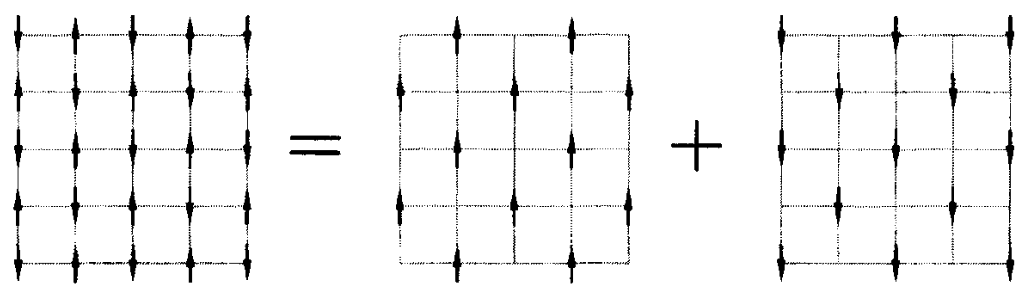
\includegraphics[scale=0.5]{images/KM2/gestaffelt.png}
    \caption{Einteilung in Subgitter.}
    \label{fig:gestaffelt}
\end{figure}\\
\end{addmargin}

\noindent\textbf{29. Was sind ein \glqq Spin-Flop\grqq\; und ein \glqq Spin-Flip\grqq \; Übergang?}\\
\begin{addmargin}[25pt]{0pt}
Legen wir ein starkes Magnetfeld an einem Antiferromagnet an. Für genügend große Feldstärken dominiert das äußere Feld und die magnetischen Momente richten sich alle parallel aus. Falls das Magnetfeld parallel zu den magnetischen Momenten angelegt wird, so bleiben sie in Reihe bei kleinen Feldstärken. Bei höheren Feldstärken hingegen nehme sie die Konfiguration wie in Abbildung (\ref{fig:Spin-Flop}) b) ein. Bei noch höheren Feldstärken werden die Winkel $\phi$ und $\theta$ immer kleiner, bis die Momente parallel zum Feld liegen. Falls aber der anisotropen Effekt groß ist, so richten sich die Momente eines Subgitters nach dem Feld aus. Es erfolgt also in einem Schritt der Übergang zur ferromagnetischen Phase.\\
\begin{figure}
    \centering
    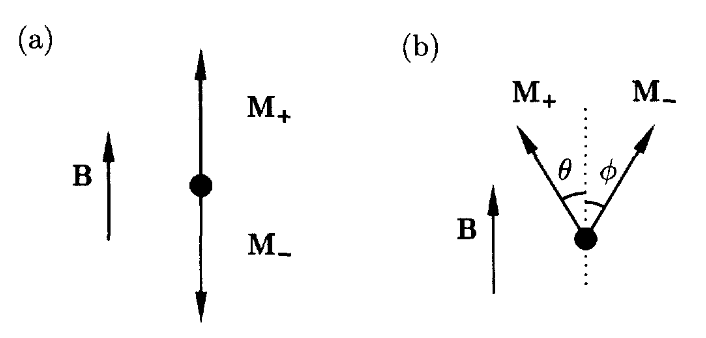
\includegraphics[scale=0.7]{images/KM2/Spin-Flop.png}
    \caption{Spin-Flop Konfigurationen.}
    \label{fig:Spin-Flop}
\end{figure}
\end{addmargin}

\noindent\textbf{30. Welche Rolle spielen Symmetriebrechungen bei magnetischer Ordnung?}\\
\begin{addmargin}[25pt]{0pt}
Symmetriebrechungen spielen eine zentrale Rolle bei magnetischer Ordnung. Sie bestimmen die Art und Weise, wie magnetische Momente in einem Material organisiert sind. Bei Phasenübergänge (z.B. von PM- zu FM-Phase) wird eine Symmetrie des Systems gebrochen.\\
\end{addmargin}

\noindent\textbf{31. Was versteht man unter einem Ordnungsparameter?}\\
\begin{addmargin}[25pt]{0pt}
Ordnungsparameter dienen der Beschreibung des Zustandes eines physikalischen Systems während eines Phasenübergangs. Wie der Name deutet ist der Ornungsparameter ein Maß für Ordnung in einem System.\\
\end{addmargin}

\noindent\textbf{32. Was versteht man unter Landau-Theorie und was unter Molekularfeldtheorie?}\\
\begin{itemize}
    \item \textbf{Landau-Theorie}: Beschreibt Phasenübergänge durch die polynomiielle Entwicklung der freinen Enthalpie als Funktion des Ordnungsparameters. 
    \item \textbf{Molekularfeldtheorie}: Ist eine Nährung, die Systeme von miteinander wechselwirkenden Teilchen als System freier Teilchen in einem externem Feld betrachtet. Das externe Feld ist als konstant angesehen (Fluktuationen werden vernachlässigt). 
\end{itemize}
\begin{addmargin}[25pt]{0pt}
    Beide Theorien sind miteinander verbindet, da die Landau-Theorie auch einen \glqq mean-field \grqq Theorie ist. Es werden also die Fluktuationen des Ordnungsparameters nicht berücksichtigt (können in Nähe des Phasenübergangs eine bedeutende Rolle spielen). 
\end{addmargin}

\noindent\textbf{33. Was versteht man unter dem Ising-Modell?}\\
\begin{addmargin}[25pt]{0pt}
Das Ising-Modell ist das Heisenberg-Modell für einer Dimension. Die Spinkomponenten können daher bloß parallel oder antiparallel zur Quantisierungsachse stehen.
\begin{equation}
    \mathcal{H}_{Ising} = -\sum_{j\neq i, i>j} J^{ij}_{A} \frac{1}{\hbar^2} (\boldsymbol{S}_{z})_{i} \cdot (\boldsymbol{S}_{z})_{j}
\end{equation}\\
\end{addmargin}

\noindent\textbf{34. Was sind Magnonen und wie sieht deren Dispersion aus?}\\
\begin{addmargin}[25pt]{0pt}
Ein Magnon ist ein kollektiver Anregungszustand eines magnetischen Systems mit Eigenschaft eines bosonischen Quasiteilchens. Für deren Disperionsrelation muss man zwischen ferro- und antiferromagnetische Phononen unterscheiden. In Gleichung (\ref{eq:Magnon-Ferr}) sieht man die quadratische Abhängigkeit für ferromagnetische Magnonen und in Gleichung (\ref{eq:Magnon-Antiff}) die lineare Abhängigkeit für antiferromagnetische Magnonen.
\begin{equation}
    \hbar \omega = 4JS(1-\cos(ka))
    \label{eq:Magnon-Ferr}
\end{equation}
\begin{equation}
    \hbar \omega \approx k
    \label{eq:Magnon-Antiff}
\end{equation}\\
\end{addmargin}

\noindent\textbf{35. Was beschreibt das Bloch'sche T hoch 3 Halbe-Gesetz?}\\
\begin{addmargin}[25pt]{0pt}
Das Bloch'sche $T^{\frac{3}{2}}$-Gesetz beschreibt den Magnonen-Beitrag zur spezifischen Wärme.
\begin{equation}
    c_{\text{Mag}} \propto T^{3/2}
    \label{eq:Bloch-T-Ges}
\end{equation}\\
\end{addmargin}

\noindent\textbf{36. Was sind magnetische Domänen und wodurch entstehen sie?}\\
\begin{addmargin}[25pt]{0pt}
Für Temperaturen unterhalb der Curie-Temperatur erwartet man, dass sich die magnetischen Momente alle parallel (oder antiparallel) bei einem Ferromagneten (Antiferromagneten) ausrichten. Beobachtet wird das nicht. Es entstehen Domänen wo innerhalb sich die Momente ausrichten, welche nicht in die gleiche Richtung zeigen. Man beobachtet also von Außen fast keine Magnetisierung. Domänen entstehen als Folge der Minimierung der freien magnetischen Enthalpiedichte (bei Ferromagneten) oder durch strukturelle Defekte (bei Antiferromagneten).\\
\end{addmargin}

\noindent\textbf{37. Was versteht man unter magnetischer Anisotropie?}\\
\begin{addmargin}[25pt]{0pt}
Magnetische Anisotropie beschreibt die Tatsache, dass magnetische MAterialien eine Vorzugsrichtung (oder Vorzugsebene) für die Magnetisierung aufweisen können. Die magnetische Anisotropie bewirkt die Kopplung der Magnetisierung an das Kristallgitter. Die magnetische Anisotropie wird von der Dipol-Dipol-WW und von der Spin-Bahn-Kopplung verursacht.\\
\end{addmargin}


\subsection{Supraleitung}
\noindent\textbf{1. Wie weißt man das Verschwinden des elektrischen Widerstandes im Supraleiter nach?}\\
\begin{addmargin}[25pt]{0pt}
Dafür verwendet man einen Ring aus supraleitendem Material und erzeugt in diesem ein Magnetfeld, die Anordnung befindet sich bei einer Temperatur oberhalb der kritischen Temperatur. Danach kühlt man das System auf $T<T_C$ und schaltet das Magnetfeld ab. Basierend auf den Erkenntnissen der Elektrodynamik würde man in diesem Ring einen exponentiell abklingenden induzierten Strom nach der Formel $I(t) = I_0 \exp\left(-\frac{Rt}{L}\right)$ erwarten. Im supraleitenden Material hingegen misst man einen nicht abfallenden induzierten Strom was zeigt, dass im Supraleiter tatsächlich exakt $R=0$ gilt. \\
\end{addmargin}

\noindent\textbf{2. Was ist der Meißner-Ochsenfeld-Effekt?}\\
\begin{addmargin}[25pt]{0pt}
Ein Supraleiter verdrängt das externe Magnetfeld komplett. Es kann dringt nur über eine Länge von $\lambda_L$ ein und wird dann von den auf der Supraleiteroberfläche erzeugten Strömen kompensiert.\\
\end{addmargin}

\noindent\textbf{3. Was unterscheidet ideale Diamagnete von Supraleitern?}\\
\begin{addmargin}[25pt]{0pt}
Antwort\\
\end{addmargin}

\noindent\textbf{4. Wie sieht das Phasendiagramm von Supraleitern aus?}\\
\begin{addmargin}[25pt]{0pt}
\begin{figure}
    \centering
    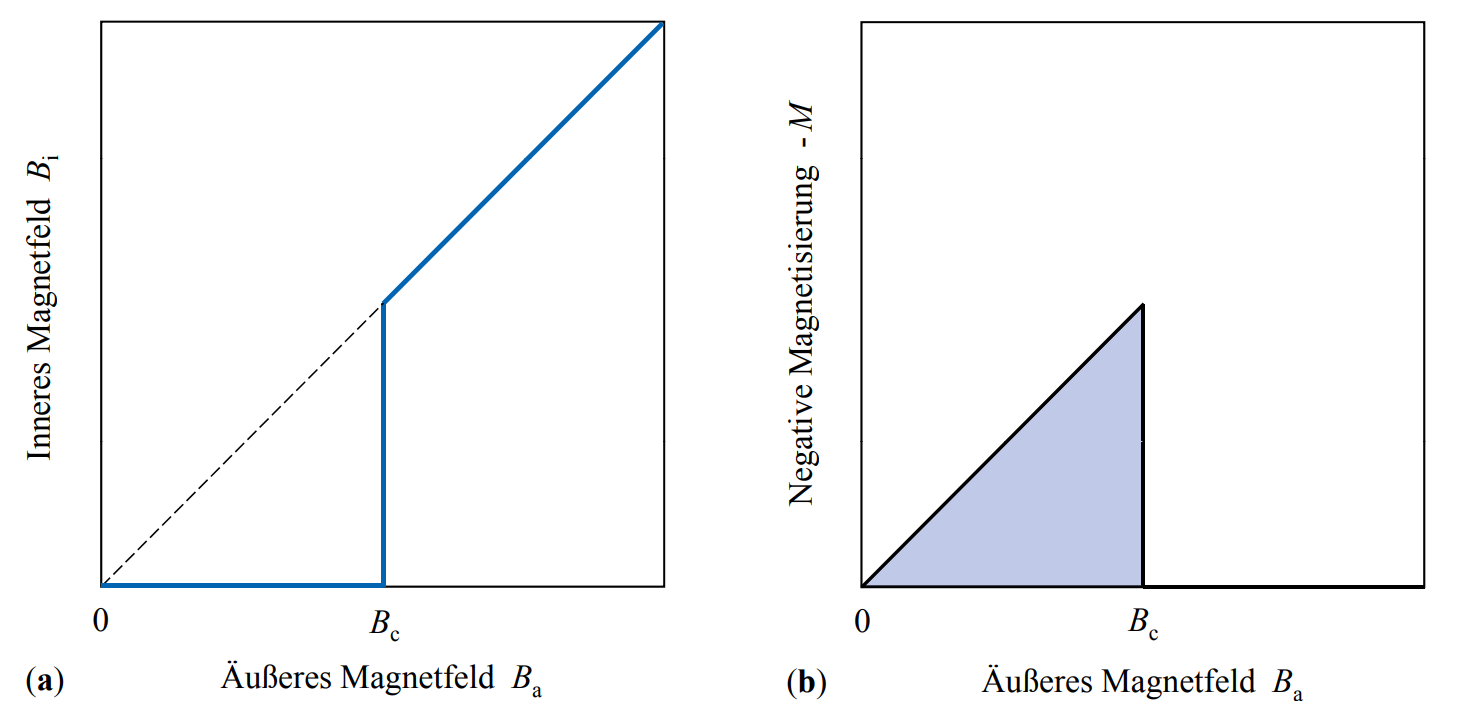
\includegraphics[width=0.7\linewidth]{images//KM2/SL_PhasendiagrammTyp1.PNG}
    \caption{Phasendiagramm eines Typ 1 Supraleiters}
    \label{fig:PhaseTyp1SL}
\end{figure}
siehe Abbildung \ref{fig:PhaseTyp1SL}
\end{addmargin}

\noindent\textbf{5. Was beschreiben die London-Gleichungen?}\\
\begin{addmargin}[25pt]{0pt}
Die London-Gleichungen sind modifizierte Maxwell-Gleichungen, die denn verschwindenden Widerstand und idealen Diamagnetismus berücksichtigen. Die 1. London-Gleichung beschreibt die Änderung des Suprastroms:
\begin{equation}
    \frac{\text{d}j_s}{\text{d}t}=\frac{n_se_s^2}{m_s}E
\end{equation}
Diese Änderung ist proportional zum E-Feld und nicht wie im Ohmschen Fall, $j_s\propto E$.
Die 2. London-Gleichung verbindet den Suprastrom mit dem abgeschirmten Magnetfeld:
\begin{equation}
    \text{rot} j_s = -\frac{n_se_s^2}{m_s}B
\end{equation}
\end{addmargin}

\noindent\textbf{6. Was versteht man unter der Londonschen Eindringtiefe?}\\
\begin{addmargin}[25pt]{0pt}
Die London-Eindringtiefe $\lambda_L=\sqrt{\frac{m_s}{\mu_0n_se_s^2}}$ ist die Länge, auf der das externe Magnetfeld auf den Wert $\frac{1}{e}$ abfällt.
\end{addmargin}

\noindent\textbf{7. Wie hängt die Enthalpie des Supraleiters vom kritischen Magnetfeld ab?}\\
\begin{addmargin}[25pt]{0pt}
Die freie Enthalpiedifferenz zwischen einem Supraleiter und einem Normalleiter beträgt $\frac{V\cdot B_c^2}{2\mu_0}$. Die freie Enthalpie des Supraleiters wird mit steigendem B also quadratisch größer.
\end{addmargin}

\noindent\textbf{8. Wie weißt man Supraleiter als thermodynamische Ordnung nach?}\\
\begin{addmargin}[25pt]{0pt}
Durch berechnen der Entropie und der daraus resultierenden spezifischen Wärme fällt auf, dass die spezifische Wärme einen Sprung bei $T_c$ hat. Damit hat ein Supraleiter einen Phasenübergang 2.Ordnung.
\end{addmargin}

\noindent\textbf{9. Was versteht man unter dem Isotopeneffekt?}\\
\begin{addmargin}[25pt]{0pt}
Eigenschaften, im Fall des Supraleiters die Sprungtemperatur, sind abhängig von der Kernmasse. Für gleiche Elemente, aber unterschiedliche Kernmassen, hat die Sprungtemperatur verschiedene Werte.
\end{addmargin}

\noindent\textbf{10. Was sind Cooper-Paare?}\\
\begin{addmargin}[25pt]{0pt}
Cooper-Paare sind attraktiv wechselwirkende Elektronen. Sie tauschen virtuelle Phononen aus. Cooper-Paare bestehen aus einem Elektron mit dem Wellenvektor $\vec{k}$ und einem Elektron mit $-\Vec{k}$.
\end{addmargin}

\noindent\textbf{11. Welcher Zusammenhang besteht zwischen Cooper-Paaren und der Gesamtwellenfunktion?}\\
\begin{addmargin}[25pt]{0pt}
Die beide Elektronen unterscheidliche Fermionen sind, muss die Gesamtwellenfunktion antisymmetrisch sein
\end{addmargin}

\noindent\textbf{12. Welche Annahme macht die BCS-Theorie über die Elektron-Elektron Wechselwirkung?}\\
\begin{addmargin}[25pt]{0pt}
Sie ist eine attraktive Wechselwirkung, die mit einer Energieabsenkung des Elektronenpaares verbunden ist.
\end{addmargin}

\noindent\textbf{13. Was zeichnet den BCS Grundzustand aus?}\\
\begin{addmargin}[25pt]{0pt}
Er existiert bei $T=0$ und es sind alle Cooper-Paare beteiligt.
\end{addmargin}

\noindent\textbf{14. Was versteht man unter der supraleitenden Kondensationsenergie?}\\
\begin{addmargin}[25pt]{0pt}
Die Kondensationsenergie ist die Energie, die durch die Bildung der Cooper-Paare gewonnen wird. Diese Energie kann für die Verdrängung des Magnetfeldes verwendet werden.
\end{addmargin}

\noindent\textbf{15. Wie hängt die Energielücke mit der Zustandsdichte zusammen?}\\
\begin{addmargin}[25pt]{0pt}
Die Energielücke ist direkt proportional zur Zustandsdichte am Ferminiveau: $\frac{E_{Kond}}{V}=-\frac{1}{4}\frac{D(E_F)}{V}\Delta^2(0)$
\end{addmargin}

\noindent\textbf{16. Wie verläuft die Dispersion ungepaarter Elektronen im Supraleiter?}\\
\begin{addmargin}[25pt]{0pt}
Die Energie eines Teilchens mit $\Vec{k}$ lautet: $E_k=\sqrt{\mu^2_k+\Delta^2_k}$. $\Delta_k$ ist hierbei die Energielücke zwischen den Cooper-Paaren und den freien Teilchen, und $\mu_k$ ist die Abweichung der kinetischen Energie der Elektronen von der Fermienergie.
\end{addmargin}

\noindent\textbf{17. Wie hängen Energielücke und supraleitende Übergangstemperatur zusammen?}\\
\begin{addmargin}[25pt]{0pt}
Es gilt (fast) Materialunabhängig
\begin{align}
    \Delta(T=0) = 1.764 k_b T_c \,.
\end{align}\\
\end{addmargin}

\noindent\textbf{18. Wie kann man die Energielücke experimentell nachweisen?}\\
\begin{addmargin}[25pt]{0pt}
\begin{itemize}
    \item speziefische Wärme: normales Metall $C \propto \gamma T$, Supraleiter $C \propto \gamma T \exp \left(-\frac{\Delta(T)}{k_b T}\right)$. Daraus folgt ein Sprung der speziefischen Wärme bei der kritischen Temperatur.
    \item thermische Wärmeleitfähigkeit: Drastische Abnahme $T << T_c$
    \item Ultraschall Absorbtion: Starke Abnahme, da weniger Stöße von Ultraschallphononen mit Elektronen.
\end{itemize}
\end{addmargin}

\noindent\textbf{19. Was versteht man unter Tunnelkontakt-Spektroskopie?}\\
\begin{addmargin}[25pt]{0pt}
Durch messen des Stroms einer Tunnelbarriere bei verschiedenen Spannungen kann auf die Zustandsdichte der beteiligten Materialien zurückgeschlossen werden. Bei genügend tiefen Temperaturen gilt die Beziehung
\begin{align}
    \frac{dI}{dU} \propto D_s(E_k = eU) \,.
\end{align}\\
\end{addmargin}

\noindent\textbf{20. Was bestimmt die kritische Stromstärke des Supraleiters?}\\
\begin{addmargin}[25pt]{0pt}
Die kritische Stromstärke wird durch das kritische Magnetfeld bestimmt. Für einen langen Draht gilt z. B.
\begin{align}
    I_c = \frac{2\pi B_c R}{\mu_0} \,.
\end{align}
Mikroskopisch kann dies dadurch erklärt werden, dass die kinetische Energie der Cooper-Paare nicht größer als die Kondensationsenergie jener werden darf.\\
\end{addmargin}

\noindent\textbf{21. Was versteht man unter Flussquantisierung des Supraleiters?}\\
\begin{addmargin}[25pt]{0pt}
In einem Supraleitenden Ring kann die Phaenverschiebung der makroskopischen Wellenfunktion nun ganze Vielfache von $2\pi$ sein. Das führt zu einer Quantisierung des magnetisches Flusses durch den Ring mit Flussquant
\begin{align}
    \Phi_0 = \frac{h}{2e} = 2.07 /cdot 10^{-15} Tm^2\,.
\end{align}
\\
\end{addmargin}

\noindent\textbf{22. Was versteht man unter dem Josephson-Gleichstrom Effekt?}\\
\begin{addmargin}[25pt]{0pt}
Durch Tunneln von Cooper-Paaren gibt es einen Stromfluss ohne Spannungsabfall. Siehe \ref{fig:Josephson_Gleichstrom}.
\begin{figure}[!h]
    \centering
    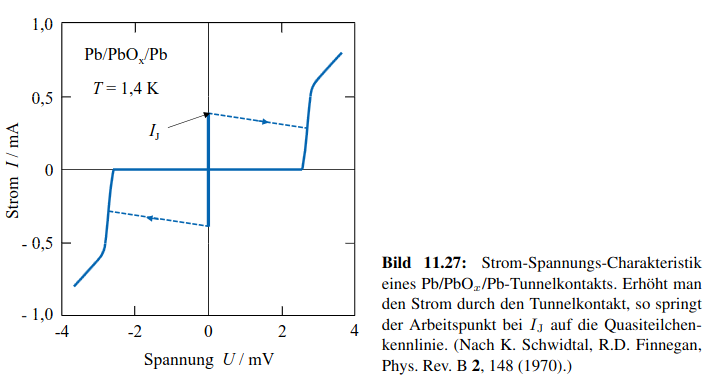
\includegraphics[width=0.7\linewidth]{images//KM2/josephson_gleichstrom.PNG}
    \caption{Strom-Spannungs Kennlinie eines Josephson Kontaktes}
    \label{fig:Josephson_Gleichstrom}
\end{figure}\\
\\
\end{addmargin}

\noindent\textbf{23. Was versteht man unter Josephson Wechselstrom}\\
\begin{addmargin}[25pt]{0pt}
Beim anlegen einer Spannung an eine Supraleitende Tunnelbarriere entsteht eine Wechselspannung ($\omega \approx 48GHz$ für $U=100\mu V$). Durch anlegen eines elektrischen Feldes wächst die Phaendifferenz der beiden makroskopischen Wellenfunktionen linear. Dies ergibt einen Wechselstrom durch die Barriere
\begin{align}
    I = I_g \sin(\omega t + \phi_0)\,.
\end{align}\\
\end{addmargin}

\noindent\textbf{24. Wie verhält sich ein Josephson-Kontakt im Magnetfeld?}\\
\begin{addmargin}[25pt]{0pt}
Für eue SQUID Schleife mit 2 Josephson Kontakten gilt
\begin{align}
    I_s \propto \cos\left(\frac{\pi \Phi}{\Phi_0}\right)\,,
\end{align}
wobei $\Phi_0 = \frac{h}{2e}$ das Flussquantum ist.\\
\end{addmargin}

\noindent\textbf{25. Was besagen die Ginzburg-Landau Gleichungen?}\\
\begin{addmargin}[25pt]{0pt}
Die GL-Theorie ist eine weiterentwicklung der Landau Theorei für Phasenübergänge 2. Ordnung, hier mit Ordnungsparameter der Copperpaar-Dichte $\eta$. Eine minimierung der freien Enthalpie führt zu den Ginzburg-Landau-Gleichungen, die den Phasenübergang der Supraleitung beschreiben.\\
\end{addmargin}

\noindent\textbf{26. Was versteht man unter Ginzburg-Landau Eindringtiefe?}\\
\begin{addmargin}[25pt]{0pt}
Die Eindringtiefe
\begin{align}
    \lambda = \sqrt{\frac{mB}{4\mu_0 e^2\lvert\alpha\rvert}}
\end{align}
\end{addmargin}

\noindent\textbf{27. Was ist die Kohärenzlänge des Supraleiters?}\\
\begin{addmargin}[25pt]{0pt}
Die Kohärenzlänge 
\begin{align}
   \xi_{GL} = \frac{\hbar}{\sqrt{2m \lvert \alpha \rvert}}
\end{align}
spiegelt die charakteristische Länge wider, über die sich die
Wellenfunktion ändern kann. Man erhält sie aus den Ginzburg-Landau-Gleichungen. Sie ist ein Maß dafür, wei schnell sich die Cooperpaar-Diche am rand aufbaut.\\
\end{addmargin}
\noindent\textbf{28. Wie ist der Ginzburg-Landau Parameter definiert?}\\
\begin{addmargin}[25pt]{0pt}
\begin{align}
    \kappa = \frac{\lambda}{\xi_{GL}}
\end{align}
mit Eindringtiefe des Magnetfelds $\lambda$ und Ginzburg-Landau Kohärenzlänge $\xi_{GL}$.
Qualitativ wägt der Ginzburg Landau parameter die Verdrängungsenergie des Magnetfelds gegen die durch Magnetfelder verkleinerte Kondensationsenergie (Cooperpaardichte) auf.\\
\end{addmargin}

\noindent\textbf{29. Was sind Typ-2-Supraleiter?}\\
\begin{addmargin}[25pt]{0pt}
Beim Typ-2-Supraleitern gibt es zwei Supraleitende Phasen. Bei niedrigen Temperaturen herrscht die Meißner-Phase vor, die auch Typ-1--Supraleitern beschreibt. Bei höheren Temperaturen ist es es allerdings bei SL 2. Art energetisch günstiger Flussschläuche auszubilden (Ginzburg-Landau-Theorie). Bei Typ 2 SL gilt $\kappa \geq \frac{1}{\sqrt{2}}$, bei Typ-1 $\kappa \leq \frac{1}{\sqrt{2}}$.\\
\end{addmargin}

\noindent\textbf{30. Wie sieht das Phasendiagramm des Typ-2-Supraleiters aus?}\\
Siehe \ref{fig:PhaseTyp2SL}.
\begin{addmargin}[25pt]{0pt}
\begin{figure}[!h]
    \centering
    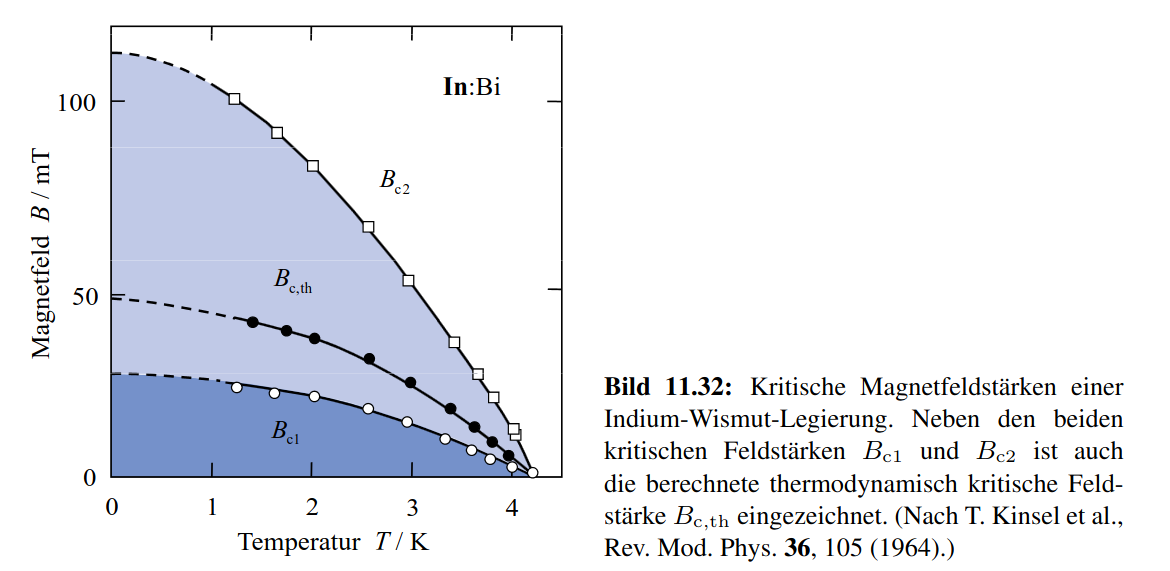
\includegraphics[width=0.7\linewidth]{images//KM2/SL_2Art_Phasen.PNG}
    \caption{Phasendiagramm eines Typ 2 Supraleiters}
    \label{fig:PhaseTyp2SL}
\end{figure} 
\end{addmargin}

\noindent\textbf{31. Was versteht man unter einem Abrikossow-Gitter}\\
\begin{addmargin}[25pt]{0pt}
Die Flusschäuche in der Schubnikov-Phase ordnen sich regelmäßig in ein Gitter an\\
\end{addmargin}

\noindent\textbf{32. Was ist flux flow?}\\
\begin{addmargin}[25pt]{0pt}
In der Schubnikov-Phase des Supraleiters 2. Art übt der Strom kraft auf die Magnetischen Flussschläuche aus. Diese bewegen sich (FLux Flow). Andererseits können diese auch durch Defekte an einen Ort gepinnt werden.\\
\end{addmargin}